\documentclass[sigconf]{acmart}

% Remove this for camera-ready
\settopmatter{printacmref=false} % Removes citation information below abstract
\renewcommand\footnotetextcopyrightpermission[1]{} % removes footnote with conference information in first column
\settopmatter{printfolios=true}

\usepackage{times}
\usepackage[utf8]{inputenc}
\usepackage{url}
\usepackage{array,multirow}
\usepackage{xspace}
\usepackage{xcolor}
\usepackage{color, colortbl} 
\usepackage{balance}
\usepackage{paralist}
\usepackage{cleveref}
%\usepackage{amssymb}
\usepackage{graphicx}
\usepackage{pifont}
\usepackage{array}
\usepackage{booktabs}
\usepackage{tikz}
\usepackage{bm}
\usepackage{enumitem}
\setlength {\marginparwidth}{2cm}
\usepackage{todonotes}
\usepackage{arydshln}
\usepackage{makecell}
\usepackage{tabularx}
\usepackage{authblk}
\usepackage{caption}
\usepackage{soul,color}
%\usepackage{subcaption}
\usepackage{mwe}
\usepackage{ifthen}
\usepackage{algorithm}
\usepackage[noend]{algpseudocode}
\usepackage{epsfig}
\usepackage[tight,footnotesize]{subfigure}

\newcommand{\cmark}{\ding{51}}%
\newcommand{\xmark}{\ding{55}}%

%!TEX root = main.tex
%=========================================================

% use true/false to toggle all comments (both kinds)

\newboolean{showcomments}
\setboolean{showcomments}{true}

% ====== comments ======
\newcommand\important[1]{\todo[inline]{\textbf{Important:} #1}}
\newcommand\alberto[1]{\todo[color=yellow,inline]{\textbf{Alberto:} #1}}
\newcommand\etienne[1]{\todo[color=orange,inline]{\textbf{Etienne:} #1}}
\newcommand\pierre[1]{\todo[color=brown,inline]{\textbf{Pierre:} #1}}
\newcommand\felix[1]{\todo[color=blue!40,inline]{\textbf{Felix:} #1}}
\newcommand\michal[1]{\todo[color=green,inline]{\textbf{Michał:} #1}}
\newcommand\onur[1]{\todo[color=red,inline]{\textbf{Onur:} #1}}
\newcommand\sergi[1]{\todo[color=pink,inline]{\textbf{Sergi:} #1}}
\newcommand\ramin[1]{\todo[color=brown,inline]{\textbf{Ramin:} #1}}
\newcommand\mustafa[1]{\todo[color=brown,inline]{\textbf{Mustafa:} #1}}
% Uncomment the following command to make all comments disappear
\ifthenelse{\boolean{showcomments}} { }
{
\renewcommand\important[1]{}
\renewcommand\alberto[1]{}
\renewcommand\mustafa[1]{}
\renewcommand\michal[1]{}
\renewcommand\onur[1]{}
\renewcommand\sergi[1]{}
\renewcommand\etienne[1]{}
\renewcommand\pierre[1]{}
\renewcommand\ramin[1]{}
}

% ====== inlined and toggable comments ======

\ifthenelse{\boolean{showcomments}}
{ \newcommand{\mynote}[3]{
    \protect\fbox{\bfseries\sffamily\scriptsize#1}
    {\small\textsf{\emph{\color{#3}{#2}}}}}}
{ \newcommand{\mynote}[3]{}}

\newcommand{\er}[1]{\mynote{Etienne}{#1}{blue}}
\newcommand{\mk}[1]{\mynote{Michał}{#1}{brown}}
\newcommand{\sr}[1]{\mynote{Sergi}{#1}{red}}

% \newcommand{\xxx}[1]{\mynote{YourName}{#1}{black!20!red!80!}}
% \newcommand{\xxx}[1]{\mynote{YourName}{#1}{green}}
\newcommand{\as}[1]{\mynote{Alberto}{#1}{orange}}
\newcommand{\dk}[1]{\mynote{Daniel}{#1}{green}}
\newcommand{\rs}[1]{\mynote{Ramin}{#1}{violet}}
\newcommand{\oa}[1]{\mynote{Onur}{#1}{red}}

% ====== systems ======
\newcommand\sysname{TOPDISC\xspace}
\newcommand\altname{DHT\xspace}
\newcommand\altsysname{PMETIS\xspace}
\newcommand\sysnamePriv{Pineapple\xspace}
\newcommand\sysnameAnon{\coconut}
\newcommand\libcoin{LibraCoin\xspace}
\newcommand\libcoins{LibraCoins\xspace}
\newcommand\privcoin{PrivCoin\xspace}
\newcommand\privcoins{PrivCoins\xspace}

\newcommand\sysnamereplay{\texttt{byzcuit}\xspace}
\newcommand\sysnamebaseline{\texttt{byzcuit-baseline}\xspace}
\newcommand\simplesysname{Simple-\sysname}

\newcommand\libra{Libra\xspace}
\newcommand\fourier{Fourier\xspace}
\newcommand\chainspace{Chainspace\xspace}
\newcommand\ethereum{Ethereum\xspace}
\newcommand\hyperledger{Hyperledger\xspace}
\newcommand\omniledger{Omniledger\xspace}
\newcommand\rapidchain{RapidChain\xspace}
\newcommand\elgamal{El-Gamal\xspace}
\newcommand\coconut{Coconut\xspace}
\newcommand\macggm{$\bm{\mathrm{MAC_{GGM}}}$\xspace}
\newcommand\sbac{S-BAC\xspace}
\newcommand\bft{BFT\xspace}
\newcommand\atomix{Atomix\xspace}
\newcommand\cscoin{CSCoin\xspace}
\newcommand\rscoin{RSCoin\xspace}
\newcommand\lsbac{\sysname}
\newcommand\fsbac{F-SBAC\xspace}
\newcommand\bftsmart{\textsc{bft-SMaRt}\xspace}

\makeatletter
\def\BState{\State\hskip-\ALG@thistlm}
\makeatother

% ====== custom notations ======
%\newcommand\algorithm[1]{\textsf{#1}}
\newcommand\hashtopoint{H^*\xspace}
\newcommand\stringtopoint{H'\xspace}
\newcommand\function[1]{\ding{118}\xspace \textsf{#1}:\xspace}
\newcommand\shard[1]{\emph{shard}\xspace#1\xspace}
\newcommand\Shard[1]{\emph{Shard}\xspace#1\xspace}
\newcommand\preacceptt{\textsf{pre-accept}($T$)\xspace}
\newcommand\preabortt{\textsf{pre-abort}($T$)\xspace}
\newcommand\preaccepttt{\textsf{pre-accept}($T'$)\xspace}
\newcommand\preaborttt{\textsf{pre-abort}($T'$)\xspace}
\newcommand\preacceptttt{\textsf{pre-accept}($T''$)\xspace}
\newcommand\preacceptts{\textsf{pre-accept}($T,s_T$)\xspace}
\newcommand\preabortts{\textsf{pre-abort}($T,s_T$)\xspace}
\newcommand\preabortttt{\textsf{pre-abort}($T''$)\xspace}
\newcommand\acceptt{\textsf{accept}($T$)\xspace}
\newcommand\abortt{\textsf{abort}($T$)\xspace}
\newcommand\accepttt{\textsf{accept}($T'$)\xspace}
\newcommand\aborttt{\textsf{abort}($T'$)\xspace}
\newcommand\acceptttt{\textsf{accept}($T''$)\xspace}
\newcommand\abortttt{\textsf{abort}($T''$)\xspace}
\newcommand\acceptts{\textsf{accept}($T,s_T$)\xspace}
\newcommand\abortts{\textsf{abort}($T,s_T$)\xspace}
\newcommand\myrow[1]{row\xspace\textsf{#1}\xspace}
\newcommand\mycolumn[1]{column\xspace\textsf{#1}\xspace}
\newcommand\shardled{shard-led\xspace}
\newcommand\Shardled{Shard-led\xspace}
\newcommand\clientled{client-led\xspace}
\newcommand\Clientled{Client-led\xspace}
\newcommand\activeObj{`active'\xspace}
\newcommand\inactiveObj{`inactive'\xspace}
\newcommand\locked{`locked'\xspace}
\newcommand\wa{{WA}\xspace}
\newcommand\wb{{WB}\xspace}
\newcommand\ka{{KA}\xspace}
\newcommand\kb{{KB}\xspace}

% ====== concepts/terminology =======

\newcommand\attacker{attacker\xspace}
\newcommand\adversary{attacker\xspace}
\newcommand\prerecorded{prerecorded\xspace}
\newcommand\prerecords{prerecords\xspace}
\newcommand\prerecord{prerecord\xspace}

%  ===== formatting ======
% Abbreviations etc.
\newcommand{\cf}{cf.\@\xspace}
\newcommand{\vs}{vs.\@\xspace}
\newcommand{\etc}{etc.\@\xspace}
\newcommand{\ala}{ala\@\xspace}
\newcommand{\wrt}{w.r.t.\@\xspace}
\newcommand{\etal}{\textit{et al.}\@\xspace}
\newcommand{\eg}{\textit{e.g.}\@\xspace}
\newcommand{\Eg}{\textit{E.g.}\@\xspace}
\newcommand{\ie}{\textit{i.e.}\@\xspace}
\newcommand{\Ie}{\textit{I.e.}\@\xspace}
\newcommand{\via}{\textit{via}\@\xspace}
\newcommand{\defacto}{\textit{de facto}\@\xspace}

\newcommand\mypara[1]{\vspace{0.05in} \noindent \textbf{#1.}}
\newcommand\para[1]{\vspace{0.05in} \noindent \textbf{#1.}}


\newcommand\definition[2]{\ding{118}\xspace \textsf{#1}\xspace$\bm{\rightarrow}$\xspace(#2):\xspace}



% For inlined section titles.
\newcommand\inlinesection[1]{{\bf #1.}}

\def\first{({\it i})\xspace}
\def\second{({\it ii})\xspace}
\def\third{({\it iii})\xspace}
\def\fourth{({\it iv})\xspace}
\def\fifth{({\it v})\xspace}
\def\sixth{({\it vi})\xspace}

\newcommand{\one}{({\em i})\xspace}
\newcommand{\two}{({\em ii})\xspace}
\newcommand{\three}{({\em iii})\xspace}
\newcommand{\four}{({\em iv})\xspace}
\newcommand{\five}{({\em v})\xspace}

% Colours
\definecolor{verylightgray}{gray}{0.8}

% Table
\newcolumntype{L}{l<{\hspace{1cm}}}
\newcolumntype{C}{c<{\hspace{1cm}}}
\newcolumntype{D}{c<{\hspace{0.3cm}}}

% Markers
\newcommand\vgap{\vskip 2ex}
\newcommand\marker{\vgap\ding{118}\xspace}

\def\na{--}
\def\unsure{?}
\def\missing{$!$}
\newcommand{\yes}{\ding{51}}
\newcommand{\no}{\ding{55}}
\DeclareRobustCommand\pie[1]{
\tikz[every node/.style={inner sep=0,outer sep=0, scale=1.5}]{
\node[minimum size=1.5ex] at (0,-1.5ex) {}; 
 \draw[fill=white] (0,-1.5ex) circle (0.75ex); \draw[fill=black] (0.75ex,-1.5ex) arc (0:#1:0.75ex); 
}
}
\def\L{\pie{0}} % Low
\def\M{\pie{-180}} % Medium
\def\H{\pie{360}} % High


\begin{document}

\title{Topic-based service discovery for the Ethereum P2P network}
\author{}


\begin{abstract}
Abstract
\end{abstract}

\maketitle

%!TEX root = ../main.tex
%=========================================================

\section{Introduction}

Ethereum~\cite{} is a decentralized, open-source blockchain with smart contract functionality, allowing the users to develop various decentralized applications (DApps),  and the most actively used blockchain~\cite{bloomberg} nowadays.
Following its decentralized design and structure, Ethereum relies on a communication infrastructure provided by a peer-to-peer (P2P) network, where individual and independent nodes, running an Ethereum client software (e.g., Go Ethereum~\cite{go-ethereum}), send and receive messages  containing transactions and blocks to achieve distributed consensus.

The set of network protocols which form the Ethereum peer-to-peer network are called DEVp2p.  DEVp2p isn't specific to a particular blockchain, but should serve the needs of any networked application associated with the Ethereum umbrella.
Other protocols can also run on top of DEVp2p,  such as 
The Whisper protocol~\cite{} (for decentralized
applications) and the Swarm protocol~\cite{} (for decentralized file
storage).
DEVp2p provides peers connection management and also node discovery services.
Between the DEVp2p network protocols and the app protocol (i.e., Ethereum, Whisper, Swarm, etc), RLPx~\cite{} provides a secure transport layer. 
\michal{The above seems too detailed IMO. We can introduce DEV2p, RLPx etc. in the background. I'd only say that Ethereum DHT can be used by other services (not necessarily blockchain related) and give some examples.}

DEVp2p manages the connections to other peers which form the overlay P2P network.
For instance,  Go-ethereum client by default establish a total of 50  connections to other Ethereum nodes.  Of these 50 slots,  two thirds are reserved for inbound connections (initiated by other peers),  while the remaining third are allocated for outbound connections. 
No further restrictions apply to inbound connections; if an inbound slot is available
Go-ethereum client simply accepts any connecting peer that supports the
Ethereum protocol and operates on the same network (main,
testing, etc.). 
The outbound slots are therefore selected by the nodes, which need to be done carefully to avoid any attacker could mount an eclipse attack.
In an eclipse attack, an
adversary monopolizes the connections of a victim, effectively
filtering the victim’s view of the blockchain.  Eclipse attacks
enable a variety of follow-up attacks such as double spending
and stubborn mining~\cite{}.
\michal{ditto}

In order to find and select participants of the P2P network to initiate connections to,  a node discovery protocol is required by DEVp2p.
Systems such as MDNS/Bonjour allow finding hosts,  but only in  a local-area network.  DEVp2p discovery protocol requires to work on the Internet and is most useful for applications with a large number of participants spread across the Internet.
There are other systems using a rendezvous server,  commonly used by desktop applications or cloud services to connect participants to each other. But using rendezvous servers requires trust in the operator and these systems are prone to censorship. 
For a decentralized network such as the Ethereum network it is not desirable to rely on a single operator.  
Instead,  it is better to place a small amount of trust in every participant, becoming more resistant to censorship as the size of the network increases and participants of multiple distinct peer-to-peer networks can share the discovery network to further increase its resilience.
The process of joining the network is the Achilles heel of the node discovery protocol: while any other node may be used as an entry point,  such a node must first be located through some other mechanism.  Approaches such as listing of initial entry points in DNS or discovery of participants in the local network can be used,  but only as a  reasonable secure entry into the network.


Current version of DEVp2p node discovery protocol is discovery version 5 (Discv5).
Node discovery protocol can be used by any node, for any purpose, at no cost other than running the network protocol and storing a limited number of other nodes' records. Any node can be used as an entry point into the network.
The system's design is loosely inspired by the Kademlia DHT~\cite{}.
In Kademlia DHT, information about known overlay nodes is stored in
a distributed table separated into so-called k-buckets (or simply buckets),  where each bucket stores nodes identifiers within the same distance to the local node id.
But unlike most DHTs no arbitrary keys and values are stored. Instead, the DHT stores and relays 'node records', which are signed documents providing information about nodes in the network. 
Node discovery protocol acts as a database of all live nodes in the network and performs three basic functions:

\begin{itemize}
 \item Sampling the set of all live participants: by walking the DHT,  the network can be enumerated.
 \item Searching for participants providing a certain service: Node Discovery v5 includes a scalable facility for registering 'topic advertisements'.These advertisements can be queried and nodes advertising a topic found.
 \item Authoritative resolution of node records: if a node's ID is known, the most recent version of its record can be retrieved.
\end{itemize}

The concept of topic is a new concept in Discv5 (compared with previous node discovery protocol Discv4).
Discv5 allows nodes to associate themselves with a set of tags, i.e., topics, and enable searching of peers that advertise themselves as associated with particular topics.  
Topics can be used to identify different  capabilities, for instance specific application capabilities,  services or certain functionalities of a node. 
\hl{Topics example missing}
Topic based peer finding is a promising feature because it allows a potential bandwidth reduction and much faster discovery of nodes
by  discovering nodes based on the topic required.
This means that instead of connecting to every node discovered to see if it offers a specific service,  we simply lookup for nodes that are only providing the service and then ask them if they really are still offering the service.
This will allow avoiding waste of time and resources by leaving apart those nodes that do not declare the service in its capabilities and avoiding handshakes node by node to discover these details and rely only on the node discovery protocol. 
\michal{I'd write the intro on a higher level. E.g., 1) Ethereum is the largest network/blockchain 2) It is fully decentralized and decentralization is great 3) Ethereum allows hosting multiple services other than Ethereum blockchain) and uses Ethereum DHT as a communication/management platform 4) A crucial part of that is to enable nodes working with the same application to find each other 5) this is challenging because of decentralization/security/malicious can join etc. 6) State of the Art doesn't work (briefly - we have better analysis in related work) 7) We propose our brand new shiny protocol that is efficiency and secure 8) Our contributions + structure}


%It is envisioned that the Discv5 system will be used across many different services at large scale, mainly to form subnetworks consisting of the service peers.  The basic objectives of Node Discovery v5 is to provide a facility for nodes to i) register 'topic advertisements', i.e., “ads”, at other peers in the Ethereum network and ii) find other nodes that advertised a particular topic by querying selected peers in the Ethereum network.

The goal of this paper is to propose and evaluate a new mechanism for the Discv5 protocol to register and discover for topics,  integrating it in the existing DEVp2p node discovery protocol based on Kademlia DHT.  
The mechanisms proposed are the following:

\begin{itemize}
 \item New registering mechanism that register nodes only for the topics that matches nodes capabilities.
 \item New table structure on top of the existing Kademlia DHT to store node information based on topics advertised.
 \item New lookup mechanism that discover nodes based on the topics advertised in the P2P network.
\end{itemize}
    
The structure of the paper is the following....\hl{TBC}


%!TEX root = ../main.tex
%=========================================================

\section{Background}
\label{sec:background}

\michal{Need a good introduction on Kademlia here. Distances/buckets etc. It's required to explain the ticket table, routing etc.}
\etienne{How different is the Ethereum Kademlia from the original published version? I can assume there have been changes in so many years. Is there a reference document for the Ethereum's Kademlia I can read?}
\sergi{From what i remember main difference are num of buckets and use of log distance.  I don't remember any document but Felix will help.}
\sergi{We should also add how kademlia is used for discovery (when lookups are performed, lookup buffer use,  pool of connections, random lookups, etc}

\subsection{Ethereum DHT}
\michal{Borrowed from \href{https://arxiv.org/pdf/1908.10141.pdf}{this paper}}
Ethereum DHT is based on Kademlia - a UDP-based, peer-to-peer distributed hash table (DHT) that is used to locate data stord in a decentralized way~\cite{maymounkov2002kademlia}. Each node is uniquely identified by its randomly generated node ID. A node ID in Ethereum is a marshaled version of node's public key. It is easy to generate many different identities but computationally infeasible to generate a specific one. A data item stored in the DHT is also found by its key, which is simply a hash of the data itself. Node IDs and data keys share the same representation; in the following we use the term ID for both.
Ethereum DHT stores data at nodes whose node ID is the “closest” to the data’s key. Closeness is defined as the bitwise XOR between two IDs, taken as an integer value, i.e.,$d(x, y) = \textit{log}_2 \lfloor x \oplus y \rfloor$.


A DHT node stores its known peers in a routing table divided into buckets which partition the known network based on the local node’s ID (\Cref{fig:kademlia}). Every bucket stores up to $k$ neighbors. Bucket $i$ stores nodes whose distance is in $[2i, 2i+1)$, which effectively corresponds to the length of the common prefix between two node IDs. The routing table stores a detailed view of peers close to the node and a less detailed view of parts of the network located further away.

Items in the DHT and nodes on the network are located by \emph{lookups}. A lookup successively queries nodes that are closest to the desired target ID (key or node ID). Intuitively, a peer closer to the target ID maintains a more detailed view of the target part of the network and provides the initial node with additional peers to query. For instance, the green node in \Cref{fig:kademlia} looking data ID in \emph{bucket 1} will ask known peers in \emph{bucket 1} that will provide additional peers closer to the data ID. Storing data follow the same process.  

\begin{figure}
    \includegraphics[width=0.4\textwidth]{img/kademlia}
    \caption{Ethereum DHT routing table.}
    \label{fig:kademlia}
 \end{figure}



%!TEX root = ../main.tex
%=========================================================

\section{System model}
We assume a network of nodes all being part of the Ethereum DHT\footnote{Currently, Ethereum DHT consist of 3,500-5,000 nodes.}. During the bootstrap process, nodes generate public/secret key pairs that are used to secure point-to-point communication with their peers (providing integrity and confidentiality). Each node is identified by its \emph{ID} (hash of the public key) and its IP address. We assume that multiple nodes may share the same IP address (due to NAT or being hosted by the same physical machine). However, no two nodes share the same ID. Nodes can play the following roles:
\begin{itemize}
    \item \textbf{Registrar} - a node that accepts registrations made by advertisers and respond to topic queries. When asked for a specific topic, a registrar should respond with advertisers that registered for the topic the registrar is aware of. All the DHT nodes play this role. Importantly, registrar may hold advertisements for multiple topics. 
    \item \textbf{Advertiser} - nodes that register for a specific topic and want to be discovered by their peers. The advertisers make themselves discoverable by placing advertisements on registrars. Nodes play a topic-specific advertiser role for every topic application it runs.
    \item \textbf{Searcher} - a node that tries to discover advertisers under a specific topic. Nodes play a topic-specific searcher role for every topic application it runs.
\end{itemize}
Multiple advertisers/searchers hosted by the same DHT node will share the same ID and IP address but will differ in topic. 

Our system indexes participants by their registered topic identifiers or topic(s), for short. A \emph{topic} is an identifier for a service provided by a node. A node providing a certain service, each identified with a topic, is said to \emph{place an ad} for itself when it registers the ad on a registrar to make itself discoverable under that topic. An \emph{ad} (\ie advertisement) is the registration of an advertiser for a topic on another node. Depending on the needs of the application, a node can advertise multiple topics or no topics at all. We assuem that the popularity of the topics in the system may vary significantly and follows a power law distribution. 

We assume the presence of malicious nodes in the DHT. The malicious nodes can freely deviate from the protocol and communicate with any other nodes in the network. The malicious node may spawn multiple virtual nodes within one physical machine and thus create multiple IDs. As creating a node requires maintaining periodic, encrypted communication with its peers, the number of active IDs an attacker can posses at a time is limited. We also assume that the number of IP addresses under the control of an attacker is limited. However, an attacker is able to generate more similar IP addresses (within a single subnet) than diverse IP addresses (with different prefixes). We use the number of IP addresses and IDs under the control of an attacker as parameters for our evaluation (\Cref{sec:evaluation}). Regardless of the number of the attacker, we assume that no honest node is fully eclipsed by the malicious ones. \textit{I.e.,} each honest DHT node has at least one honest peer. 


\section{Design Goals}\label{sec:goals}

The topic table is shared across multiple advertisers and stores topics with varying popularity (which is determined by how many nodes register the topic) among the participants of Discv5. It is important that the high popularity of a particular topic should not prevent peers from registering less popular topics. This is achieved using the waiting time function discussed below.



Under the assumption listed above, we target to achieve the following goals:
\begin{itemize}
    \item G1 - all the registrants (regardless of the topic they register for) should be able to place their advertisements in the network. Aka no registrants can be globally denied registrations.
    \item G2 - all the registrants within each topic should have a similar probability of being discovered by their peers.
    \item G3 - the load (in terms of sent and received messages) should be equally distributed across all the nodes regardless of their ID and location in the network
    \item G4 - the registration operation should be efficient in terms of time (fast) for all the registrants
    \item G5 - the registration operation should be efficient in terms of overhead (low amount of sent/received messages) for all the registrants
    \item G6 - the lookup operation should be efficient in terms of time (fast) and messages sent (hop count) for all the query nodes
    \item G7 - the number of total registrations per topic should be proportional to the popularity of the topic (the number of registrants).
    \item G8 - the protocol should be resistant to network dynamic (nodes joining leaving)
    \item G9 - the protocol should be resistant to sybil attacks lanched by malicious nodes
\end{itemize}

%!TEX root = ../main.tex
%=========================================================

\section{Overview}

There are 2 main operations, register(topic, self) and lookup(topic)
Every node acts as a advertiser and a registrar

\sergi{I would merge section 5 and 6 into a single section following the same structure of https://github.com/datahop/p2p-service-discovery/blob/master/doc/specs.md}

\subsection{Register}
Every registrar holds a \emph{topic table}, where it stores the incoming ads (\Cref{fig:registration}). Advertisers can send their requests to be added to the topic table on a registrar. Upon reception of a registration request, registrars compare it against ads already present in the table and calculates a request-specific \emph{waiting time}. The waiting time is determined by the diversity score of the incoming request and the occupancy of the topic table. The more the request differs from ads in the table, the lower waiting time it receives. It allows to maintain diverse content of the topic table, protects against hijacking the table by a small number of advertisers and ensures fairness towards less popular topics in the system. As the topic table gets filled, the returned waiting times increase as well. It spreads the load equally across registrars (loaded registrars issue longer waiting times and slow down the incoming traffic) and limits the total ad number in the table (bounding the registrar memory usage). 

A request is admitted to the table only if its \emph{accumulated waiting time} is higher than the returned waiting time. The \emph{accumulated waiting time} represents the total time the advertiser already waited for admission and is registered in \emph{ticket}. Tickets are immutable objects issued and signed by the registrars and includes the time of the initial request sent by the advertiser and the last waiting time returned by the registrar. Using the tickets avoids keeping additional state on registrars, while allows the advertisers to prove their \emph{accumulated waiting time}. 

If the \emph{accumulated waiting time} is lower than the waiting time, the advertiser receives a new ticket, waits for the remaining waiting time (waiting time - accumulated waiting time) and retries the registration. Importantly, the waiting time is re-evaluated every time the advertiser comes back. I.e., a previously returned waiting time is not an obligation for the registrar to admit the request at the specified time. The system guarantees that advertisers that waited long enough will eventually register at the topic table. 

\begin{figure}
    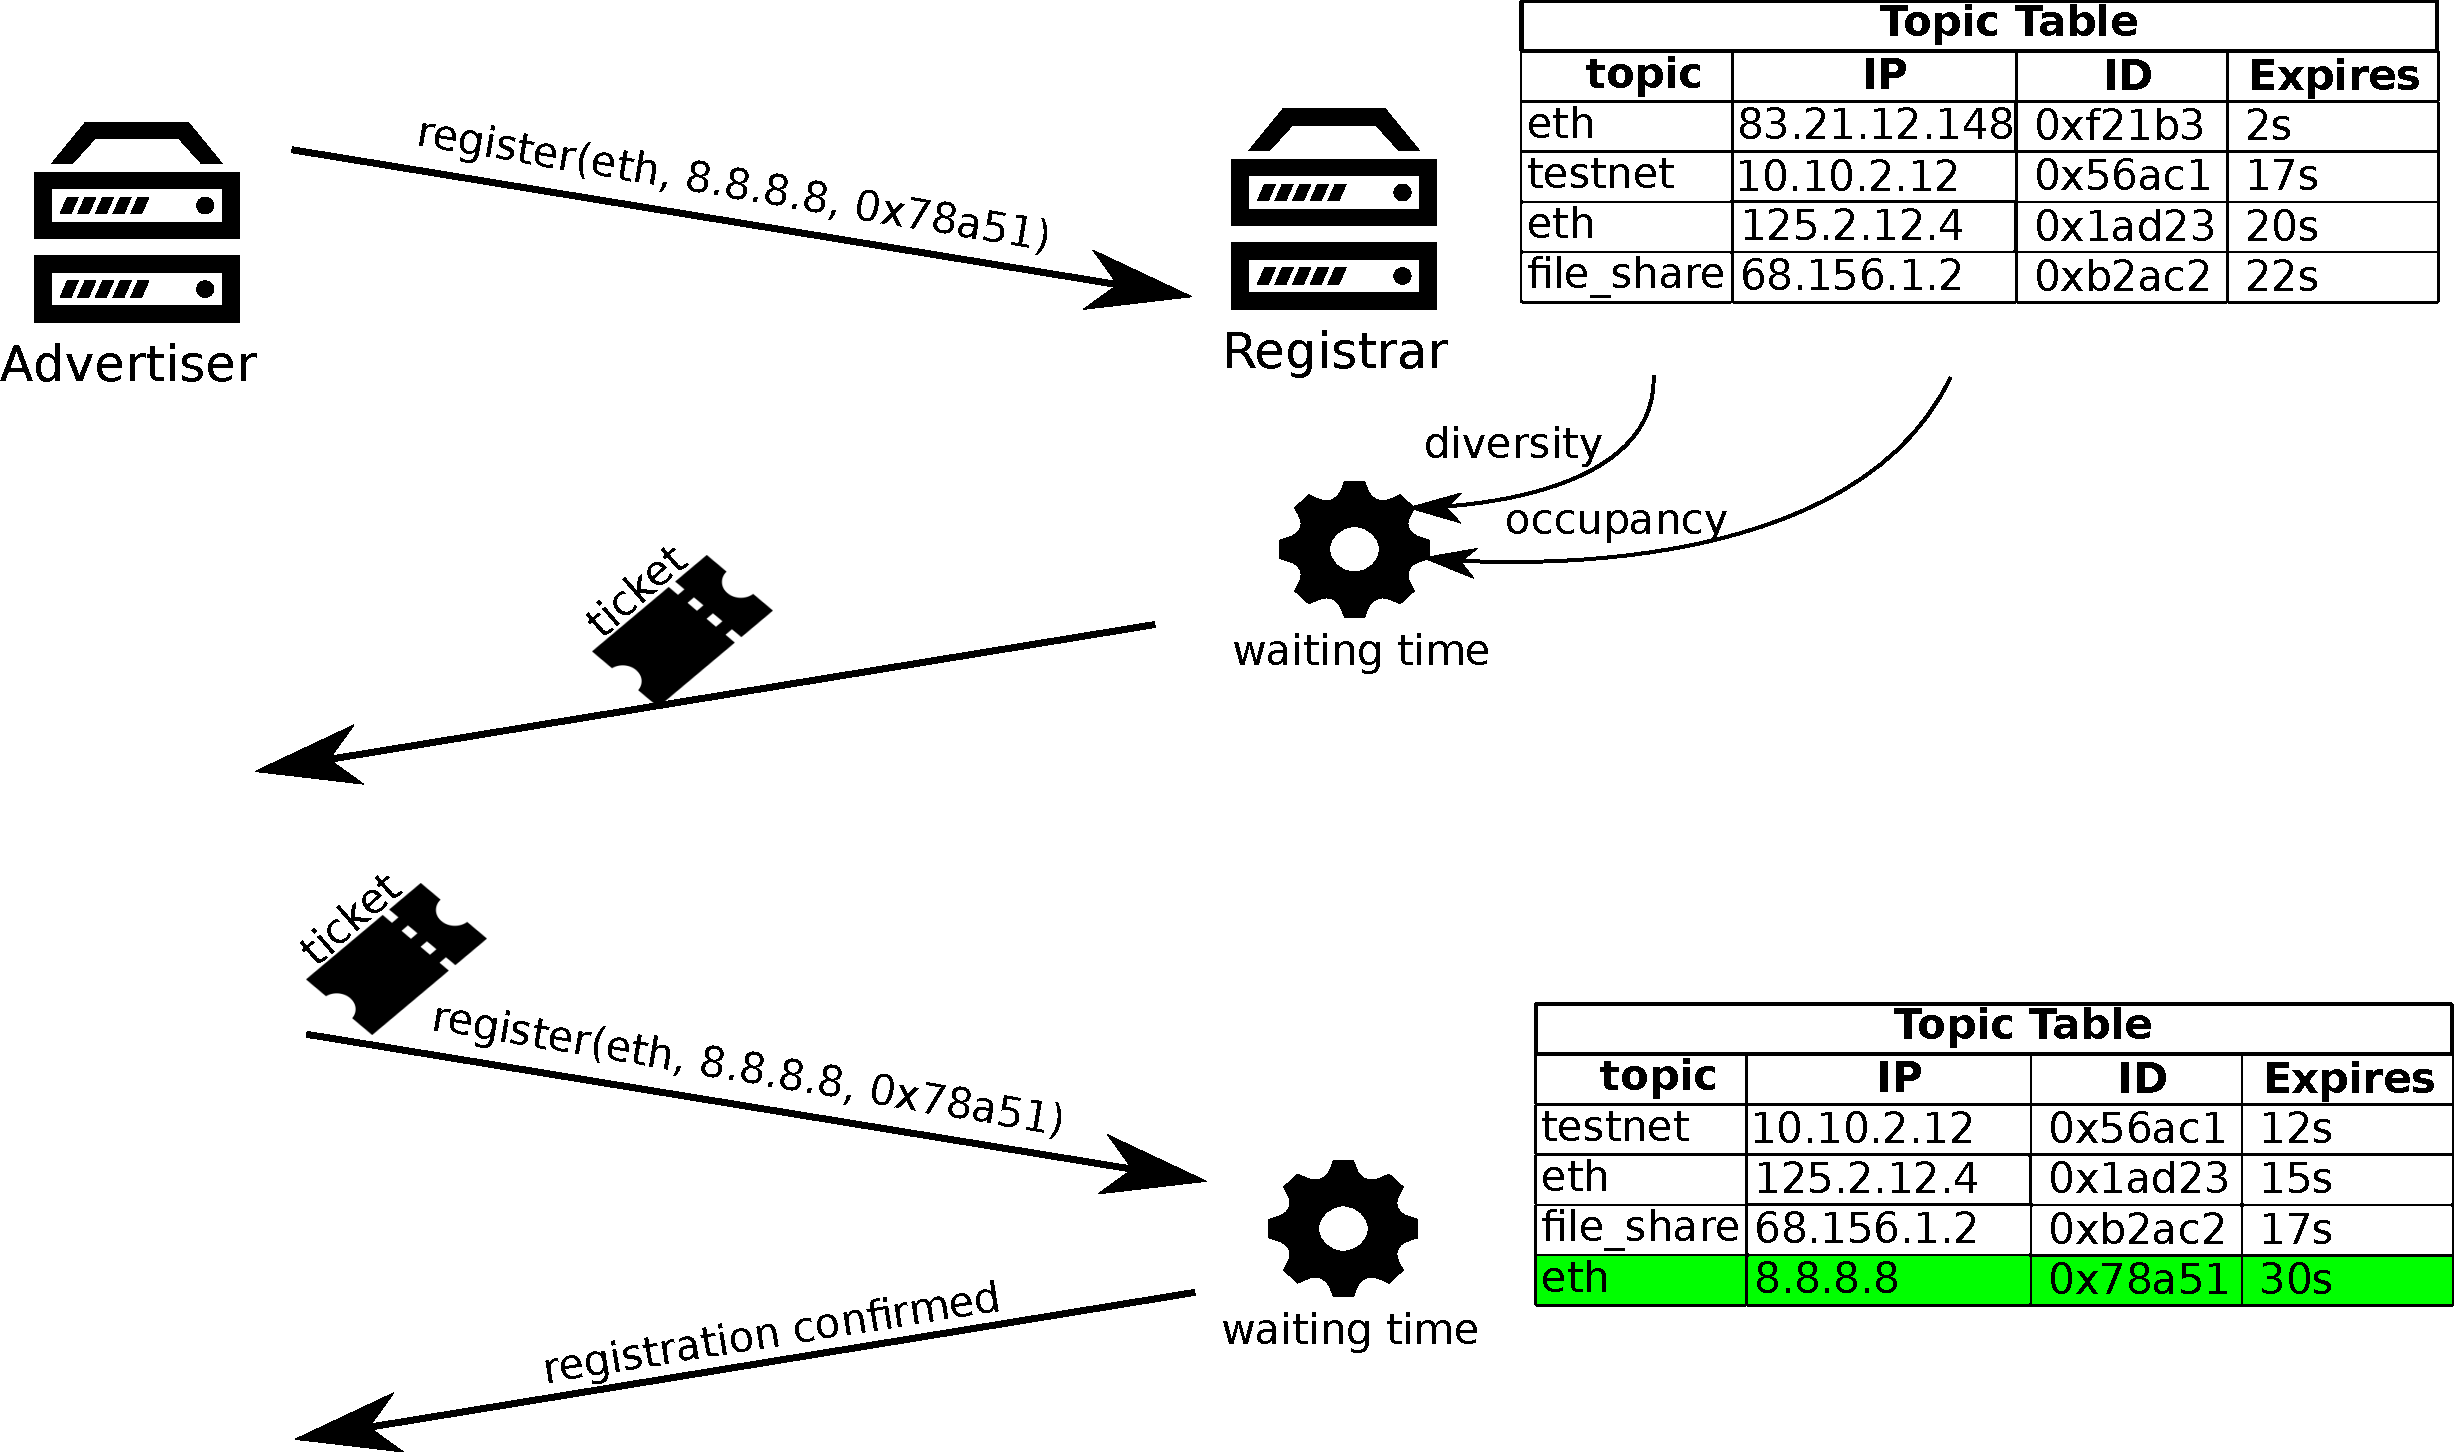
\includegraphics[width=0.5\textwidth]{img/registration}
    \caption{Registration process within one registrar.}
    \label{fig:registration}
\end{figure}




During the registration process, each advertiser tries to place its ads on multiple advertisers. It is required for availability as a single registrar can be malicious, attacked or simply leave the network. The advertisements should be placed in an unpredictable way to avoid targeted attack. On the other hand, the relevant registrar should be easy to find for searchers. Finally, we want to minimize the number of placed advertisement due efficiency reasons. 

At the beginning of each registration operation advertisers construct a \emph{ticket table} that will lead the process. The \emph{ticket table} is similar to the routing table. It is divided into buckets and holds peers in each bucket. However, buckets in the \emph{ticket table} indicate the distance from the topic hash the advertisers wants to register. The \emph{ticket table} is initialized with advertisers' peers from the DHT routing tables but organized in a different way (\Cref{fig:ticket_table}). The advertisers then tries to registers at a fixed number of registrars per bucket in the \emph{ticket table}. If a bucket holds more than the required number of registrars, a random subset is selected by the advertiser. The registration operation, places topic advertisements only on a small subsets of nodes (low overhead), includes randomness when choosing the registrars (attack resistance) and goes towards a specific point in the network indicated by the topic hash (efficient lookup).

Initially, advertisers might not know any nodes in buckets close to the topic hash\footnote{Especially if the topic hash is "far away" from the advertiser's ID}. When responding to registration requests, registrars also include a fixed amount of the closest peers to the topic hash the registrars know. The advertiser uses this information to progressively fill its ticket table. The closer the advertiser gets with the registration process, the more detailed information it receives. Similarly, to the basic DHT routing process, the registration operation eventually leads to the registrar that is the closest one to the topic hash in the entire network. 

\begin{figure}
    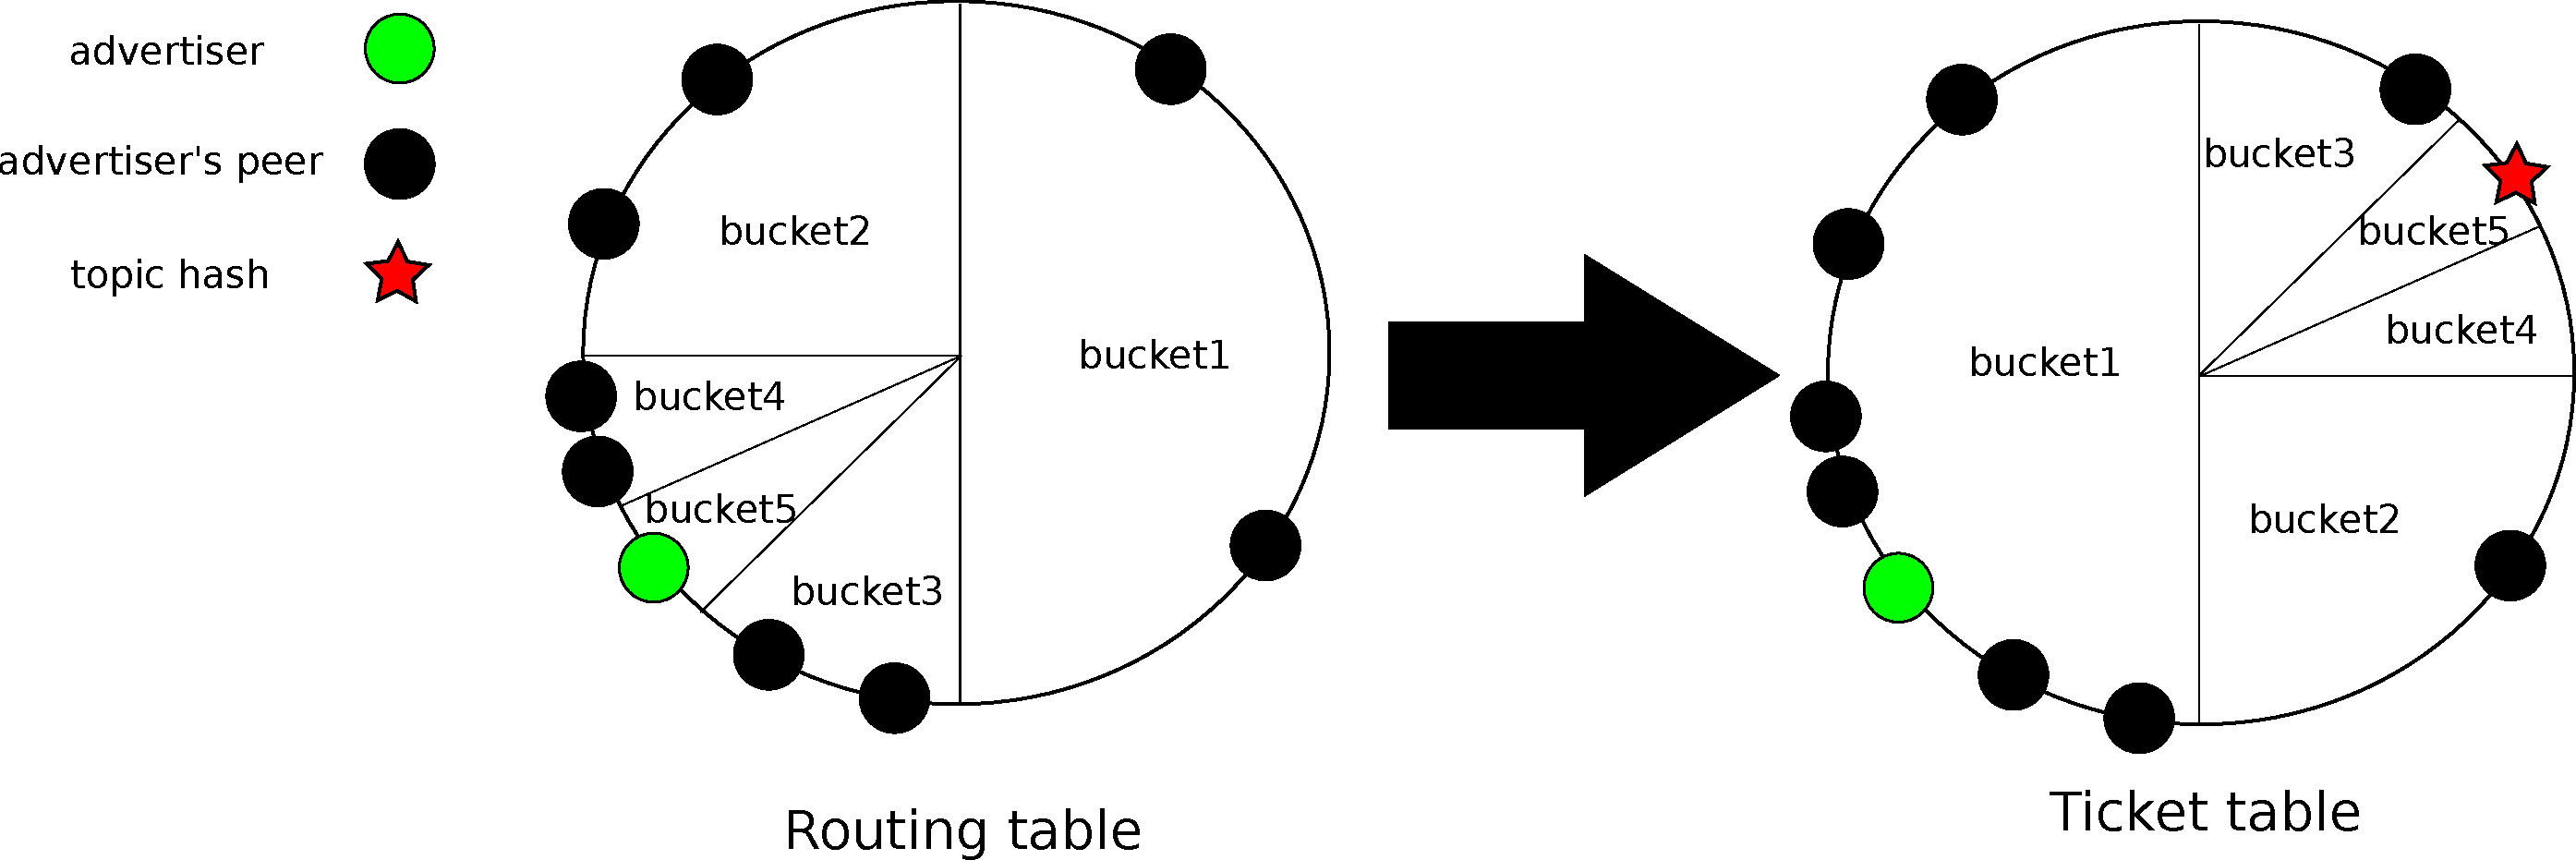
\includegraphics[width=0.5\textwidth]{img/ticket_table}
    \caption{Creation of ticket table from the routing table.}
    \label{fig:ticket_table}
\end{figure}

\subsection{Lookup}
The lookup operation closely mirrors the registration operation. The searcher starts by creating a \emph{search table}, organized in the same way as the \emph{ticket table} and determined by the topic hash. The searcher then starts the search from the furthest buckets in the search table and progressively moving towards buckets closer to the topic hash. A fixed number of random registrars is contacted for each bucket. Similarly to the registration operation, queried registrars respond with a list of the closest peers to the topic hash the registrars know of, allowing to progressively populate the search table. The search process stops when enough peers were found or when the closest registrar to the topic hash is reached. This approach allow searcher of popular topics to stop the process after a few queries without going all the way towards the topic hash and improves the load balance in the system. On the other hand, searchers of less popular topics are guaranteed to eventually discover all peer subscribed to their topic. 



\section{Design}

\subsection{Topic Table}

\subsection{Tickets}
In order to place an ad on a registrar's topic table, the advertiser must present a valid 'ticket' to the registrar. Tickets are immutable objects issued by the registrars. An advertiser willing to register an ad at a registrar must first obtain a ticket from that registrar by sending a 'ticket request' (TICKETREQUEST) message to the registrar. In response to the ticket request, the registrar issues an initial ticket containing a 'waiting time' and sends the ticket to the advertiser in a 'ticket response' message. The advertiser can come back to the registrar (to register an ad) after the waiting time has elapsed and present the ticket in a 'topic registration request' (i.e., REGTOPIC) message.

Any REGTOPIC messages that are sent before the waiting time (indicated in the ticket) are ignored by the registrars. If the advertiser comes back to the registrar after the waiting time, the advertiser can either place the ad (and notify the advertiser of a successful registration) or issue another ticket with a new waiting time in another ticket response message. An advertiser may be given one or more tickets in a sequence before a successful registration, and this means that overall the advertiser waits for a 'cumulative waiting time' period that is the sum of multiple waiting times issued in each ticket in the sequence before finally registering an ad. Assignment of 'waiting times' is the only way the registrars can control the registrations in order to both:

\begin{itemize}
    \item Throttle ad placement rate to prevent overflowing of topic table: when the topic table is full, the advertisers must wait for already placed ads to expire first before they are allowed to register new ads.
    \item Prioritise registrations to achieve a diverse set of ads in the topic table. For example, registrations for less popular topics or registrations from advertisers that increase IP diversity (in the set of advertiser IP addresses that currently have an ad in the table) can be prioritised over others. This is useful to reduce the impact of Sybil attacks on the service discovery system.
\end{itemize}

Waiting times will be calculated according to a 'Waiting time function' (see below). Enforcing this time limit prevents misuse of the topic table because any topic must be important enough to outweigh the cost of waiting for ad placement. Imagine a group phone call: announcing the participants of the call using topic advertisement isn't a good use of the system because the topic exists only for a short time and will have very few participants. The waiting time prevents using the topic table for this purpose because the call might already be over before everyone could get registered. Also, it prevents attackers from overflowing topic table by regulating registrations in case of spamming attacks.

In addition to the waiting time, the sequence of tickets issued by a registrar for a specific advertiser also records the original issue-time of the first ticket which can be used to compute the cumulative waiting time so far; that is, the time elapsed since the advertiser requested its first ticket to place its ad. The inclusion of issue-time allows the registrars to prioritise advertisers that have been waiting the most as we explain later. Because the tickets are immutable (i.e., tampering with the ticket is detectable by the registrars that originally issued the ticket), when a registrar issues a new ticket (in case a registration is not immediately successful) to an advertiser, the registrar simply copies the issue-time from the last issued ticket and use that as the issue-time of the new ticket. This means that the registrars are not required to maintain any state for each on-going ticket request given that they can simply verify the authenticity of the ticket in the incoming registration requests. The registrars ensure the authenticity of the tickets they issue to the advertisers through symmetric encryption we explain below.

Tickets are immutable objects storing arbitrary information determined by the issuing registrar node. While details of encoding and ticket validation are up to the implementation, tickets must contain enough information to verify that:
\begin{itemize}
    \item The advertiser attempting to use the ticket is the one which originally requested it.
    \item A ticket is valid for a single topic only.
    \item A ticket can only be used within the 'registration window' (explained below).
    \item A ticket can't be used more than once.\michal{Can we enforce it? I can use the same ticket twice within the validity period, right?}
\end{itemize}

Tickets cannot be used beyond their lifetime. If an advertiser does not come back after the waiting time, all cumulative waiting time is lost and the advertiser must start over (\Cref{fig:ticket_validity}). When the ticket is issued, the node keeping it must wait until the registration window opens. The length of the registration window is implementation dependent, but by default 10 seconds is used. The ticket becomes invalid after the registration window has passed. This mechanism prevent from malicious advertisers who could get ticket, wait for a long time generating high cumulative waiting time and launching a coordinated attack to take over the topic table.
    
    
\begin{figure}
    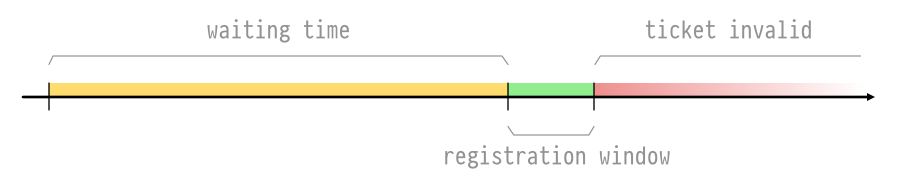
\includegraphics[width=0.5\textwidth]{img/ticket-validity}
    \caption{Ticket validity period.}
    \label{fig:ticket_validity}
\end{figure}

\subsection{Ticket Table}
The above description explains the storage and placement of ads on a single registrar, but the advertisers need to distribute ads redundantly on multiple nodes in order to speed up its discovery and to be discovered by more searchers at once. The main goal of distributing advertisements to be found within the network. An important issue is how advertisers distribute their ads among registrar nodes. Since every node may act as an advertisement medium for any topic, advertisers and searchers looking for ads must somehow meet at common registrars. Ideally, the topic search should be fast even when the number of advertisers for a topic is much smaller than the number of all live nodes. Given that in a decentralised setting, advertisers and registrars can not apriori agree on a subset of nodes to serve as the advertisement media for the topics, the main challenge for nodes is to find the "right" set of nodes to send advertisements and topic search queries so that they quickly meet at common nodes.



In order to execute the ad distribution process described below, each advertiser maintains a per-topic 'ticket table' for each topic it is advertising to keep track of the ongoing registration attempts with different registrars. This table is similar to the routing table used in Kademlia protocol, but instead of storing nodes based on distance for routing purposes, nodes are stored based on distance to topic ID to keep track of on-going registrations.

This table is made up of k-buckets of logarithmic distance to the topic hash (topic ID), i.e. the table stores k registrars for every distance step (bucket). It is sufficient to use a small value of k such as k=3. For this table no replacement list is used, different from the Kademlia routing table. Ticket table buckets are filled from the local routing table (Kademlia DHT Table) with the same distance to the topic hash.

Every node stored in the ticket table is a potential registrar. The advertiser attempts to place an ad on each registrar and keeps the latest ticket issued by that registrar. It also keeps references to all pending tickets in a priority queue keyed by the expiry time of the ticket so it can efficiently access the next ticket for which a placement attempt is due.

In our approach, advertisers start a limited number of parallel registrations in each ticket table bucket distance. More specifically, an advertiser follows the below steps to distribute its ads for a specific topic:
\begin{enumerate}
    \item The advertiser selects a set of K registrar nodes from each bucket distance of the ticket table structure, where the number of bucket distances (B) is a configurable parameter of the ticket table.
    \item A TICKETREQUEST message is initially sent to each of the selected registrar nodes in the previous step.
    \item Registrar node replies with a TICKETRESPONSE. This message includes the TICKET which contains a waiting time and a ticket issue time.
    \item The advertiser replies after the waiting time expires with a REGTOPIC request containing the previously received TICKET attached to it.
    \item A registration is successful when the waiting time calculated at the registrar is smaller than the cumulative waiting time, which means that the advertiser has waited long enough.The registrar sends a \item REGCONFIRMATION response to the advertiser. In general, the topic table occupancy is guaranteed to always remain below the topic table capacity by the waiting time calculated: the waiting time function returns increasingly large values as the topic table space runs out; the waiting time becomes infinite in case there is no space.
    \item The registrar replies with a REGRESPONSE message containing a new TICKET (containing a new waiting time) in case the registration is not succesful.
    \item A registrar gives up and stops the registration process with a registrar (say R) upon either T unsuccessful registration attempts (i.e., after being issued T tickets in REGRESPONSE messages from the registrar without a REGCONFIRMATION) or receipt of a ticket with a waiting time larger than LARGEWAIT. In that case, the advertiser selects a new node located in the same bucket as R, and initiates a TICKETREQUEST (step 2).
    \item Similarly, expiration of a previously placed ad (i.e., after the passage of ad-lifetime upon receiving a REGCONFIRMATION message) also triggers TICKETREQUEST to a new node that is in the same bucket as R.
\end{enumerate}

The objective of the ad placement process described above is to establish and maintain K active (i.e., unexpired) registrations in each bucket distance. This objective is achieved by the advertisers setting a timer with a duration of ad-lifetime immediately upon the receipt of a REGCONFIRMATION from a node in a bucket b, and once the timer expires (after ad-lifetime passes) the advertiser starts a fresh registration with a node that is also located in bucket b. The ticket table is used to store the tickets obtained for each on-going registrations and to keep track of the expiration times of active registrations.

\subsubsection{Bucket refresh}

The Ticket table needs to be initialised and refreshed to fill up all the per-distance k-buckets. Ideally, all k-buckets should be constantly full, meaning that the advertisers place registrations at registrars in all distances to the topic hash. An option to fill up all k-buckets would be to send periodic lookups for the specific distance to the topic hash, but since there are some distances that tend to be empty in the id space, sending periodic lookups for the topic hash may create an additional overhead that can be too expensive and create too much traffic in the network. To avoid that, initially, the 'ticket table' k-buckets are filled performing local DHT routing table lookups to all distances to the 'topic hash' of the advertised topic.

In addition to that, every time a node sends a ticket or registration request, the registrar replies with the closest nodes to 'the topic hash' that it knows. This helps filling up k-buckets without sending additional lookups. Also, when performing topic search (sending lookups for specific topics), closest known nodes to 'the topic hash' are attached by the registrar node in the response.

There is also a refresh bucket process, similar to the Kademlia DHT table, where periodically a random bucket is checked for empty buckets. The refresh time used is $refresh_time=10$ seconds. During the refresh process, the empty slots can be filled from the local DHT table list, and optionally a lookup (Kademlia FINDNODE) can be performed towards the topic hash. Also, all nodes in the bucket are periodically pinged to check they are still alive. In case they are not, tickets for those dead nodes are removed from the ticket table and registrations to new nodes are initiated.


\subsection{Waiting Time}
Waiting time function is used to calculate the waiting time reported to registering advertising nodes to regulate and control the ticket registration. The function directly shapes the structure of the topic table, determines its diversity and performs flow control. The function should also protect against all kinds of attacks, where a malicious actor tries to exhaust resources of the registrar. At the same time, no hard limits on the advertiser IPs/IDs/registered topic should be imposed, allowing the table to be used in various environments.

The waiting for a specific request follows the formula below (we assume that the ads contain advertiser IP, ID and topic):


\begin{equation}
    w=((\frac{1}{10^9}) + (\frac{d(IP)}{d})^{P_{IP}}+(\frac{d(ID)}{d})^{P_{ID}} (\frac{d(topic)}{d})^{P_{topic}}) \frac{ba}{(1-\frac{n}{d})^{P_{occupancy}}}
\end{equation}

All the modifiers from the first part of the equation increase with increasing number of the same items that are already in the table, i.e., reduction in diversity. Thus it's getting increasingly difficult to register ads for the same IP/ID/topic. For instance, ads for less popular topic will receive lower waiting times than popular ones. Note that the table does not prevent anyone from registering, but rather makes it slower for already popular items. Such a mechanism promotes diversity in the table and protects against Sybil attacks so that an attacker who is in control of a limited pool of IP addresses won't be able to dominate the table with many ads. The low exponent for the topics is motivated by the topics in the network that are likely to follow a skewed (e.g., a zipf-like) distribution. In contrast, honest nodes' IPs/IDs should follow a uniform distribution.

The latter part of the formula is determined based on a multiple of ad-lifetime and the current utilisation (i.e., occupancy divided by capacity) of the table. When the utilisation becomes closer to 1.0, the base time becomes very large due to a very small denominator. Before the waiting time becomes infinite (when utilisation becomes 1), the waiting time becomes extremely high, in which case the advertisers give up as explained in the ad distribution process.

\subsubsection{Lower Bound}

With the formula above, user are incentivized to keep checking the waiting time as frequently as possible hoping for a better one. An advertiser may get a better waiting time at t2 if an contribuing to the waiting time received at t1 (t1 < t2) expires before t2. One solution to this problem is to take into account all the expiration times when calculating the waiting time. However, such a solution is computationally expensive (O(n)) and unfeasible in practice.

We thus enforce a lower bound on the waiting time. I.e., we make sure that a searcher's waiting time received at t2 is not smaller than the waiting time at t1 by more than w(t1) - w(t2) < t2 - t1. To achieve that we split the above formula into topic/IP/ID distinctive parts:



The waiting time is equal to: 

For each of the components above IP, ID and topic present in the table, we keep a bound. When a specific IP enters the table for the first time, the bound(IP) is set to 0 and a timestamp timestamp(IP) is set to the current time. When a ticket request arrives from the same IP, we calculate the IP waiting time $w_{IP}$ and return the higher value among $w_{IP} = max(w_{IP}, bound(IP) - timestamp(IP))$. It makes sure that advertisers never receive a better time by frequently coming requesting new tickets. The bound and the bound are updated when a new ticket is issued and $w_{IP} > (bound(IP) - timestamp(IP))$. The same holds for IDs and topics.


\subsection{Topic Lookup}
The purpose of placing ads is to be discovered by searchers. Searchers maintain a separate table that they use to keep track of on-going searches called the 'search table'. Similar to the 'ticket table', the search table also stores k-buckets of advertisement media by distance to the topic hash, and a new 'search table' is created for each topic lookup. The k factor of the search table should be relatively large in order to make the search efficient. By default we use k=16 similarly to the Kademlia DHT. Tickets are not required for search and nodes can not be added multiple times in the same k-bucket.

To find ads, the searcher simply queries the nodes in the search table for ads. In order to find new results, bucket entries are replaced when the node fails to answer or when it answers with an empty list of ads. Bucket entries of the search table should also be replaced whenever the table is refreshed by a lookup.

\subsubsection{Search strategy}

For the lookup process, we perform ALPHA=3 parallel lookups to three different nodes. In case not enough LOOKUP\_LIMIT=50 results have been received for the first ALPHA lookups, additional ALPHA parallel lookups are performed until reaching LOOKUP\_LIMIT or MAX\_LOOKUP\_HOPS=50. We implemented and evaluated the following strategy in order to choose which nodes from which buckets ask first when performing a lookup. A random node is picked from a bucket following a round-robin approach. It starts picking a random node from the highest distance bucket and follows to the next distance in the bucket list.

\subsubsection{Bucket refresh}

Similarly to 'ticket table', 'search table' needs to be initialised and refreshed to fill up all the per-distance k-buckets. Ideally, all k-buckets should be constantly full, making it possible to query any distance to the topic hash. Since there are some distances that tend to be empty in the id space, sending periodic lookups for the topic hash my create and additional overhead that can create too much traffic in the network. To avoid that, initially, 'search table' k-buckets are filled performing local DHT routing table lookups to all distances to the 'topic hash'. In addition to that, every time an advertiser sends a ticket request and when performing topic search at a registrar, the registrar replies with the closest nodes to 'the topic hash' that it knows, helping to fill up the k-buckets of ticket tables without advertisers sending additional (Kademlia FINDNODE) lookups.

There is also a refresh process, similar to the Kademlia DHT table, where periodically a random bucket is checked for empty buckets. The refresh time used is refresh\_time=10 seconds. When empty slots during the refresh process, optionally, lookups are performed to the topic hash in case is empty. Also, the last node in the bucket is pinged to check it is still alive. In case it is not, it is removed from the table.

%!TEX root = ../main.tex
%=========================================================

\section{Performance Evaluation}
\label{sec:eval}
%
%In  this  section,  we  provide  a  detailed  investigation  of  the performance of the proposed discovery scheme.
%We present the performance evalution in three different subsections. 
%In the first one we evaluate the performance of our novel waiting function by measuring the ticket table occupancy
%according with our design goals and parameters.
%The second one is a thorough performance evaluation under different scenarios, including Sybil attacks, of the whole network discovery solution using a peer-to-peer network simulator.
%In the third one we include an evaluation using the most used Ethereum client software, Geth~\cite{go-ethereum}, in a testbed scenario.

%\subsection{Ticket table occupancy evaluation}

%\sergi{Ticket table occupancy and waiting time evaluation TBC}

%\subsection{Network simulator evaluation}

%\sergi{TODO: modify figures with bigger fonts}
%\sergi{TODO: registrant distribution is not very readable. probably should be redesigned}
%\sergi{TODO: Lookup performance should be compared with something. Discv4? }

\subsection{Evaluation Setup}

For the  performance evaluation of the proposed discovery scheme. we extended the existing  large-scale peer-to-peer network simulator PeerSim~\cite{p2p09-peersim}.
We implemented the current Discv5 protocol by modyfing the available PeerSim Kademlia implementation with the differences of the Kademlia version used by the Ethereum network, and developing our solution on top of it. 
We make the code publicly available for the scientific community\footnote{https://github.com/datahop/p2p-service-discovery}.

\begin{table}[!hbt]
\centering
\scriptsize
\begin{tabular}{|c|c|}%|c|c|}
\hline
Parameter     & Value (\%) \\
\hline
\hline
%Network size & 2000 nodes \\%&  0.4321 & 0.8883\\
%\hline
Simulation time & 4 hours \\%& 0.7569 & 0.9959\\
\hline
Kademlia bucket size & 16 \\%& 0.6104 & 0.8515\\
\hline
Kademlia buckets & 17 \\%& 0.8225 & 0.9897\\
\hline
Ticket table bucket size & 5 \\%& 0.8225 & 0.9897\\
\hline
Ticket table buckets & 10 \\%& 0.8225 & 0.9897\\
\hline
Lookup table bucket size & 16 \\%& 0.8225 & 0.9897\\
\hline
Lookup table buckets & 17 \\%& 0.8225 & 0.9897\\
\hline
Registration lifetime & 15 minutes \\%& 0.8225 & 0.9897\\
\hline
Registration waiting time limit & 15 minutes \\%& 0.8225 & 0.9897\\
\hline
Number of topics & 5 \\%& 0.8225 & 0.9897\\
\hline
Number of topics & 5 \\%& 0.8225 & 0.9897\\
\hline
Zipf dist exp & 0.7 \\%& 0.8225 & 0.9897\\
\hline
Ticket table capacity & 500 \\
\hline
Turbulence event & Every 144 seconds per 1000 nodes. \\%& 0.8225 & 0.9897\\
\hline
Num of connections & 50 \\%& 0.8225 & 0.9897\\
\hline
\bottomrule
\end{tabular}
\vspace{2mm}
\caption{Evaluation scenario parameters}
\label{tab:param}
\vspace{-0.05in}
\end{table}

In Table~\ref{tab:param} we show the parameters used in the simulation. 
We performed 4 hours long simulations with different number of nodes from 500 to 10000.
In the simulations there are 5 different topics and all nodes participate in at least one topic (t1).\michal{We need simulations with more topics. 5 is just not enough.}
There is turbulence in the simulation,  \ie new nodes are added to the network and existing nodes are removed at a rate of one event every 144 seconds per each thousand nodes in the network.\michal{We 144? Do we have any churn data from Ethereum?}
Nodes are modelled similarly to an Ethereum client. 
When a node joins the network it starts advertising for the participating topics.
Each node has a pool of connections (separated by outgoing and incoming connections) for each topic in which they participate, and it perform lookups
for a specific topic to start connections with discovered nodes.
When an initial lookup is done,  the discovered nodes are stored in a buffer per topic.
Nodes start attempting connections with the discovered nodes from the buffer until all connections  are full.
In case the connection is possible (the targeted node has an available slot in the pool of connections and the node is still up), it is added 
to the local list of connections.
Nodes are removed from the discovered nodes buffer for each attempt of connection.
When a node goes down, a connection attempt is made with a new nodes from the buffer to occupy all available connection slots.
When the discovered nodes for a certain topic is empty, a new topic lookup is performed.
Nodes have a pool of 50 connections available, 16 for outgoing connections and 34 for incoming.

%\begin{table}[!hbt]
%\centering
%\scriptsize
%\begin{tabular}{|c|c|}%|c|c|}
%\hline
%Topic & 500 Nodes & 1000 Nodes & 5000 nodes & 10000 nodes \\
%\hline
%\hline
%T1 & 500 nodes & 1000 nodes & 5000 nodes & 10000 nodes \\%&  0.4321 & 0.8883\\
%\hline
%T2 & 1272 nodes \\%& 0.7569 & 0.9959\\
%\hline
%T3 & 803 nodes \\%& 0.6104 & 0.8515\\
%\hline
%T4 & 496 nodes \\%& 0.8225 & 0.9897\\
%\hline
%T5 & 218 nodes \\%& 0.8225 & 0.9897\\
%\hline
%\bottomrule
%\end{tabular}
%\vspace{2mm}
%\caption{Nodes per topic}
%\label{tab:nodes}
%\vspace{-0.05in}
%\end{table}


%\subsubsection{Results}

%\paragraph{\bf{Active registrations}:}

\subsection{Performance Results}
\michal{We should group the result so that they show achievement of specific goals that we described before}

%\paragraph{Ticket registrations:
In the following we detail the performance evaluation in four different subsections.  In the first we show the registration performance.  Secondly we show the traffic load and overhead of the designed mechanism.  Then we continue with the lookup and discovery performance and we finish with the security analysis.

\subsubsection{Registration  performance}

In Figure~\ref{fig:regs} we observe the average active registrations in the system per topic with different number of nodes in the simulation,  from 500 to 10000 nodes. 
We can observe nodes for all topics are able to place a substantial amount of registrations, even the less popular topics. 
As number of nodes increase in the network, we can observe the differences between registrations per topic are reduced. 
Actually, it can be observed the most popular topic (t1) is able to place less registrations than t2. 
This is caused by the fact that with more nodes trying to register for the same topic,  waiting times increase.
If the waiting time increases over the waiting time limit (in the simulations is set to 15 min),  the node cancels the registration and tries with a different nodes.
When cancellations happen it may lead to less active registrations, because it may end up with longer registration processes.
In our simulation we observe less registrations for t1 than t2  because t1 registrations waiting time go over the waiting time limit more often.

In Figure~\ref{fig:time_reg} we observe the average time necessary for a node to place a registration,  from 500 to 10000 nodes in the simulation.
We can observe that average registration time is always below 500 seconds and this is reduced for less popular topics and smaller networks. 
This figure does not include registration times for cancelled registrations.
\sergi{I think we should include failed/uncomplete registrations in the plot}

\begin{figure}[!h]
\centering
\subfigure[{Active registrations}]{
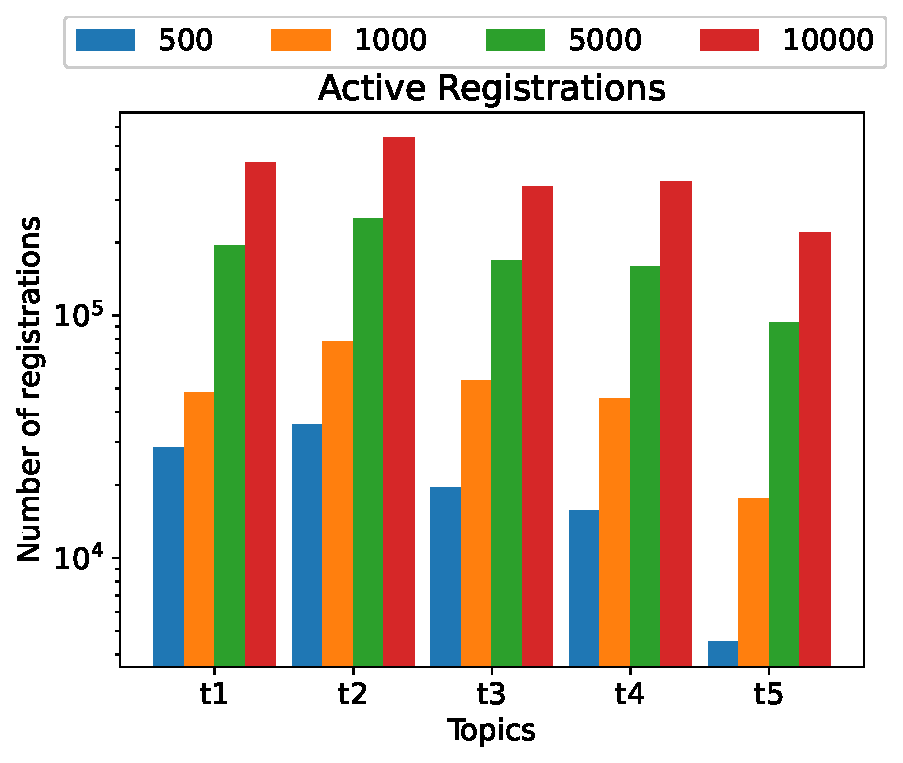
\includegraphics[width=0.225\textwidth]{img/eval/registration_origin.eps}
\label{fig:regs}
} 
\hspace{-0.25cm}
\subfigure[{Time to register}]{
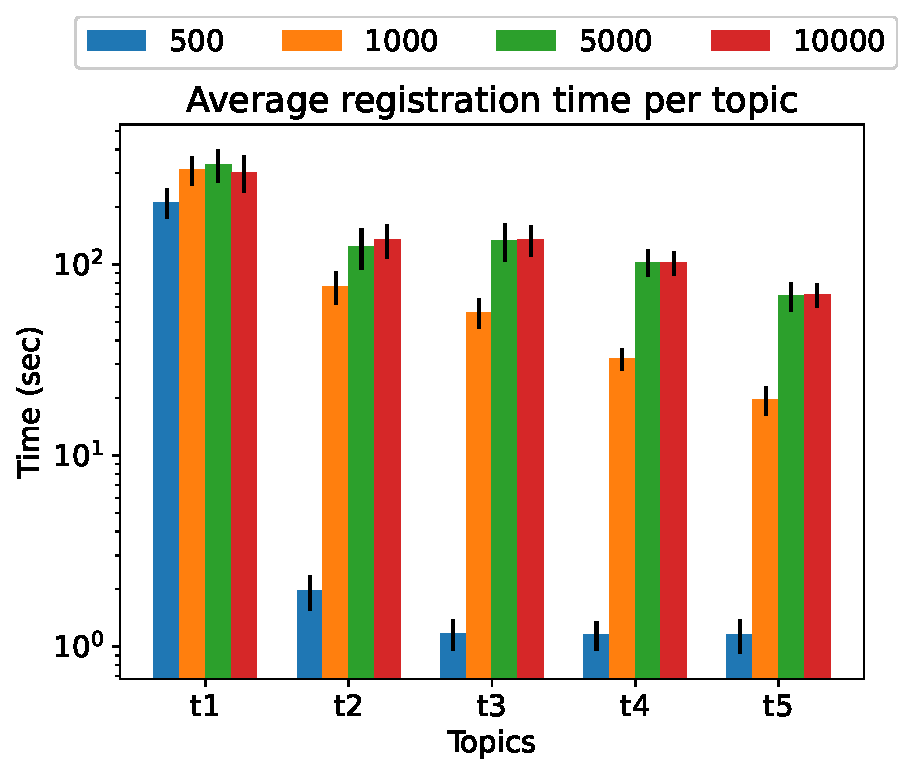
\includegraphics[width=0.225\textwidth]{img/eval/avg_time_register.eps}
\label{fig:time_reg}
}
 \caption{Ticket registrations} 
\label{fig:registrations}
\vspace{-0.15in}
\end{figure}   

%\begin{figure}[h!]
%\centering
%%\epsfig{file=imgs/eval/scen5.pdf, width=0.45\textwidth}
%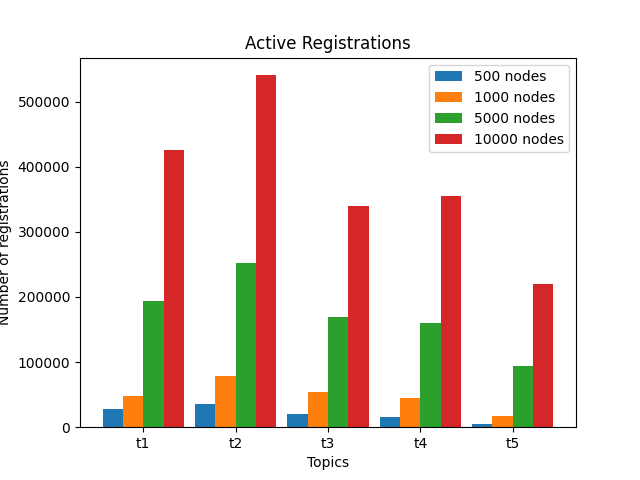
\includegraphics[width=0.225\textwidth]{img/eval/registration_origin.png}
%\caption{Registrations}
%\label{fig:regs}
%\vspace{-0.15in}
%\end{figure}

%\paragraph{\bf{Network load}:}
\subsubsection{Network load}

In Figure~\ref{fig:messages}~and~\ref{fig:msg_distr} we can observe the traffic load generated in the network.
In Figure~\ref{fig:messages} we observe most of the messages are ticket requests/replies, and the subsequent registration request/replies
after receiving a ticket from a node. 
This is caused by the fact that nodes are constantly registering dynamically. 
In Figure~\ref{fig:msg_distr} the messages received distribution. 
We can observe some nodes receive much more messages.
This is caused by the bucket node distribution, where nodes with identifiers close to topic hash ids receive more initial tickets requests because there are less.
However, we observe while the number of nodes in the network is increased 20 times,  the  maximum number of messages received by some nodes does not increase in the same way,  only being twice the amount when comparing 500 with 10000 nodes,  ans with increases lower than 30\% when number of nodes are doubled.
Moreover,  we can also see the number of messages received does not exceed 10 times the average value of the messages received. 

Therefore, the system is able to scale without danger of overloading some of the nodes of the network.

\begin{figure}[!h]
\centering
\subfigure[{Number of messages}]{
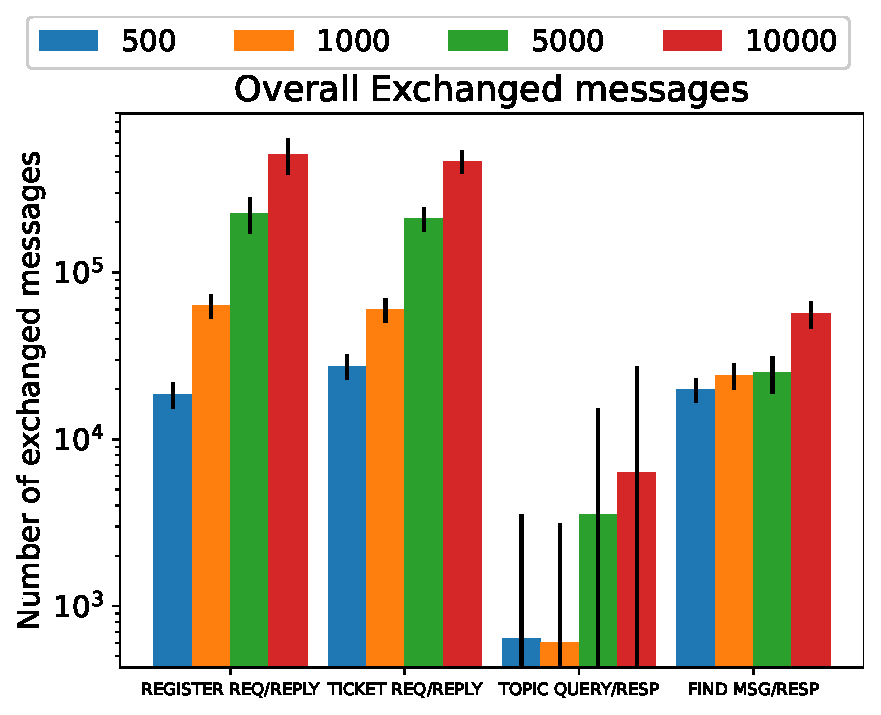
\includegraphics[width=0.225\textwidth]{img/eval/message_quantity.eps} 
\label{fig:messages}
} 
\hspace{-0.25cm}
\subfigure[{Message distribution}]{
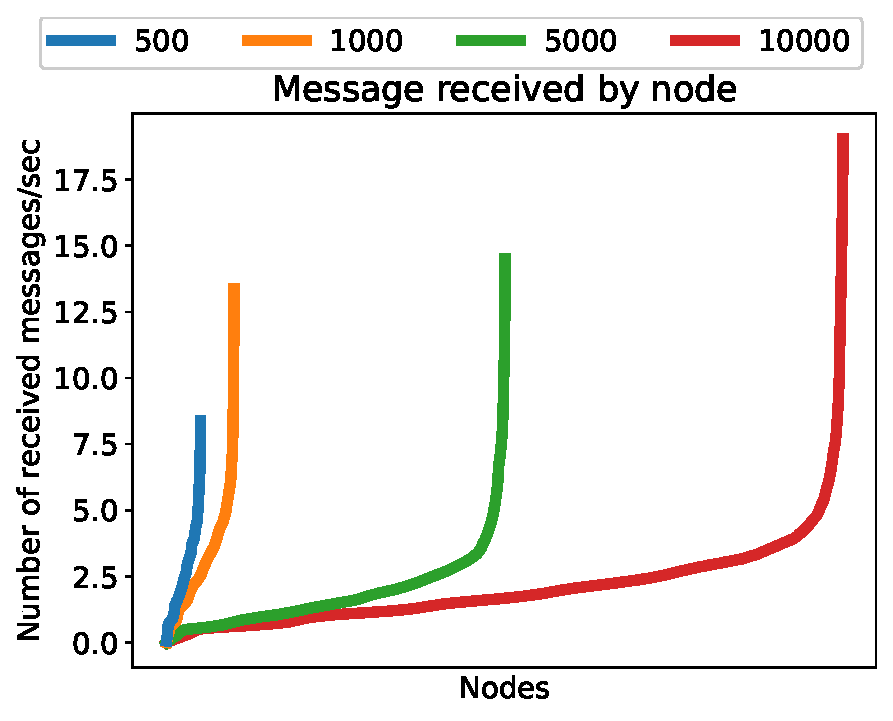
\includegraphics[width=0.225\textwidth]{img/eval/messages_received.eps} %\hspace{-1.5em}%
\label{fig:msg_distr}
}
 \caption{Traffic load} 
\label{fig:traffic}
\vspace{-0.15in}
\end{figure}   

\subsubsection{Discovery and lookup performance}

%\paragraph{\bf{Discovery performance}:}

In Figure~\ref{fig:reg_disc} and \ref{fig:timedisc} we can observe how nodes are discovered within the network.
In Figure~\ref{fig:reg_disc} we observe the percentage of the nodes in the network that are discovered and how often are discovered.
Each node in the network is represented by a circle, and the size of the cirle represents the relative frequency of discoveries compared with other nodes in the network.
We can observe that for all topics the percentage of nodes discovered in the network is very close to 100\%. This means almost all nodes in the network are able to be discovered by other nodes. The number of dicovered nodes is not 100\% because of the existence of turbulence (there are some nodes just joined the network and there has not been enough time yet to be discovered). In case there are a low number of nodes for a specific topic (e.g. t5 with 500 nodes network) the 100\% is reached.
We can also observe Figure~\ref{fig:reg_disc} that the discovery distribution is bounded to \hl{X} times between the most discovered and the least discovered.
We observe the dots size are very regular and despite being not completely equal the differences are not substantial. 
In Figure~\ref{fig:timedisc} we observe the time between a registration is completed and the first time the registration
is returned in a lookup.
By observing this we can see how difficult is for a node to be discovered once is able to place a registration. 
We see the average time is between 20 and 10 seconds in most of the cases, except for the least popular topic t5 which is around 50\% higher. 
We also observe the deviation is bounded at around 60 seconds, with equivalent different for t5.


\begin{figure}[!h]
\centering
\subfigure[{Registrant discovery distribution}]{
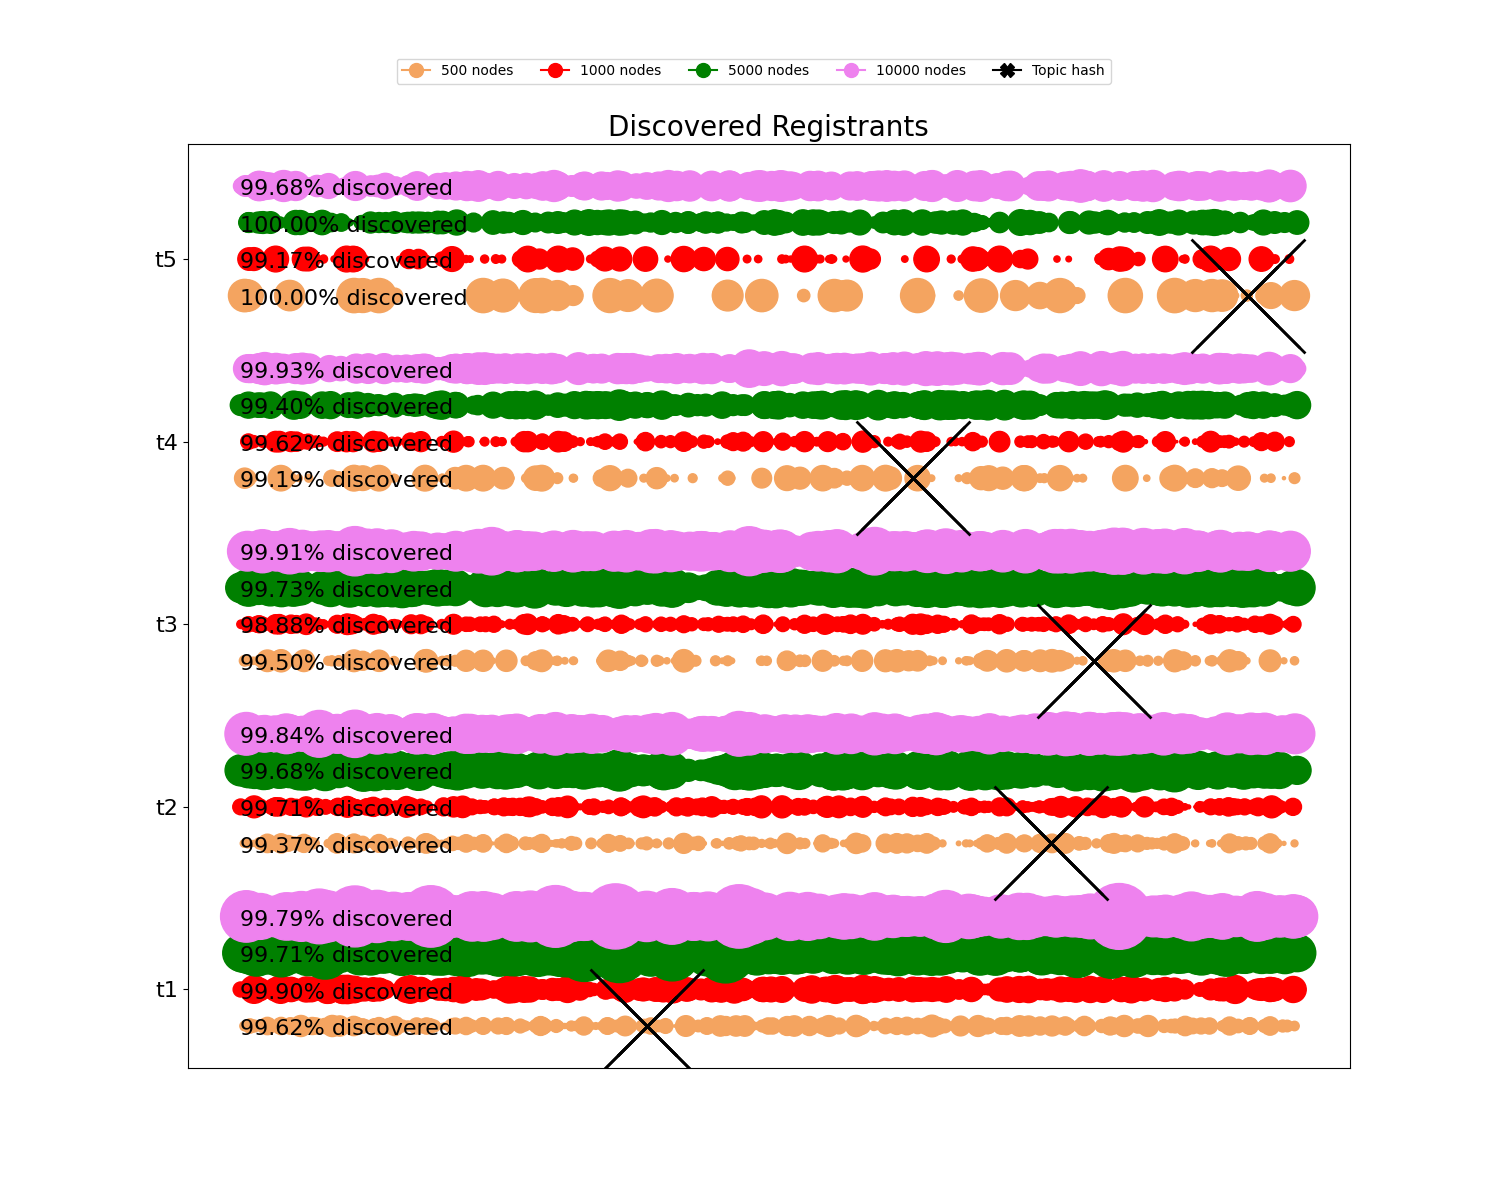
\includegraphics[width=0.225\textwidth]{img/eval/registrant_distribution.eps} 
\label{fig:reg_disc}
} 
\hspace{-0.25cm}
\subfigure[{Time between registration and first discovery}]{
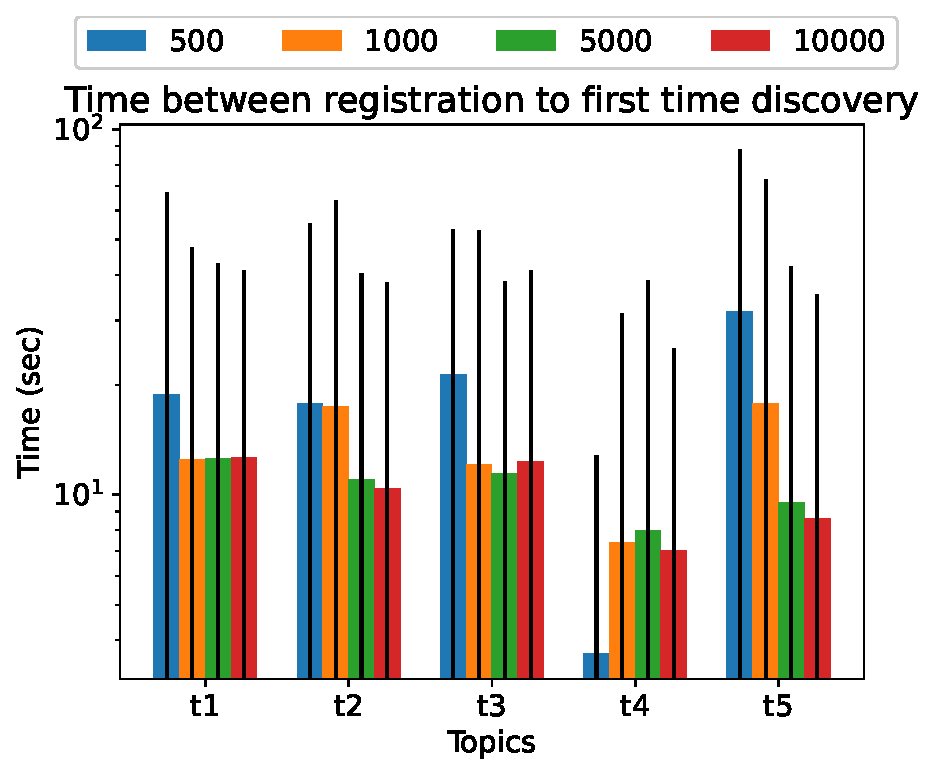
\includegraphics[width=0.225\textwidth]{img/eval/min_time_discovery.eps} %\hspace{-1.5em}%
\label{fig:timedisc}
}
 \caption{Discovery performance} 
\label{fig:discovery}
\vspace{-0.15in}
\end{figure}   


In Figure~\ref{fig:hopcount} we can observe the lookup performance of \sysname compared with Discv4 for a 5000 nodes simulation.
In the plot we show the average number of nodes discovered for each hop during a lookup per topic, taking into account that Discv4 cannot do per topic lookups,  so we discard received nodes that do not support the specific service.
In the figure we observe that for t1 the discovered nodes are higher when using Discv4, since all topics support t1 and any node discovered will be a valid node. 
However, as the popularity of the topic decreases it also does the lookup performance of Discv4,  since it is very difficult to find nodes for non-popular topics without supporting per topic lookups.
In this sense,  Discv5 lookup performance also decreases the performance with non-popular topics (simply because there are less nodes in the network) however this decrease is diminished.  Between t1 and t5 the lookup performance is decrease approximately to a 1/2th for Discv5, while when using Discv4 the lookup performance decreased to a less than a 1/10th.

%TODO add lookup description including mechanisms to avoid sybils.

\begin{figure}[h!]
\centering
%\epsfig{file=imgs/eval/scen5.pdf, width=0.45\textwidth}
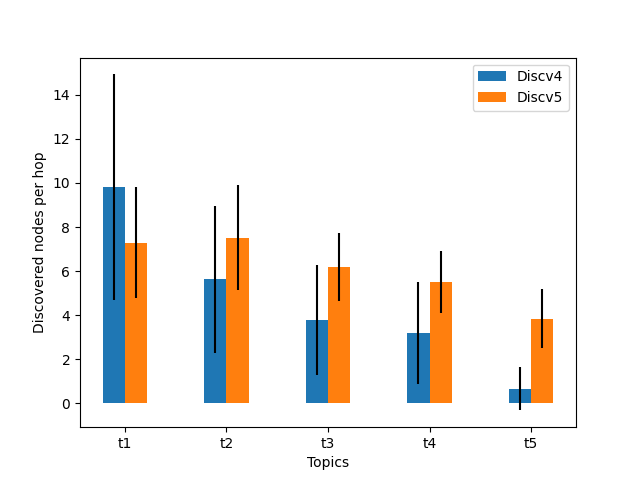
\includegraphics[width=0.35\textwidth]{img/eval/lookup_hopcount_discv4.png}
\caption{Lookup performance}
\label{fig:hopcount}
\vspace{-0.15in}
\end{figure}

\subsubsection{Sybil Attacks}

In the following we show the results of the performance evaluation of the discovery service under different sybil attacks.  The attacks that we evaluated in this section are of two types and are previously described in Section~\ref{sec:overview}. 
These attacks are eclipsing  and Denial-of-service (DoS) attacks.
Eclipsing attacks goal is to generate multiple fake identities within a topic to be able to eclipse existing nodes in the network.
Eclipsing a node imply all outbound and inbound connections are established to only sybil/fake nodes controlled by an attacker.
This allows the attacker to control the view of the network of the eclipsed node and can be used to co-opt a victim's mining power and use it to attack the blockchain's consensus algorithm.
DoS attacks instead is an attack meant to hamper the good performance or even to shut down the network, making it inaccessible to its intended users.  
In our case,  the goal of DoS attacks is to difficult or to block the discovery of nodes in the network and is specially important for topic with low popularity where finding all node in the network is very important.

In the implemented topic eclipsing attack,  malicious nodes are sybil nodes that cooperate in order to eclipse other valid nodes.
Malicious and valid nodes have the same amount of bandwidth resources and malicious nodes respond to topic lookup requests and find messages with only other malicious nodes.
Malicious nodes also act as evil 'registrants' trying to place as many registrations as possible by using bigger ticket size,  with malicious registrars attack,  where evil registrars replies with only malicious nodes when receiving a topic query.

We implemented and evaluated two kind of DoS attacks.  
The first attack consists in a topic spam attack where a big number of sybil identities generated try to register for non-existing random topics.
By registering for non-existing topics,  evil nodes try to harm valid topics registrations, overflowing topic tables.
The second DoS attack consists on generating sybil identities that keep without replying when receiving valid nodes ticket requests or return very long waiting times. 
This way an attacker can try to backlog valid nodes ticket registrations.

In Figures~\ref{fig:reg_eclipse},~\ref{fig:discoverytime_eclipse}~and~\ref{fig:lookup_eclipse} we show performance results under a
topic eclipsing attack.
We compare results for topic eclipsing attacks targeted to the most popular topic (t1) and attacks targeted to the least popular topic (t5). 
In the simulation there are 2000 nodes, all of them participating in t1 and only 218 participating in t5. 
In the simulations there are an additional 20\% (400 in total) malicious nodes that target the specific topic and the number of resources used in the attack (IP addresses) vary from 1 address to 50.

\begin{figure}[!h]
\centering
\subfigure[{Active registrations eclipse attack t1 attack}]{
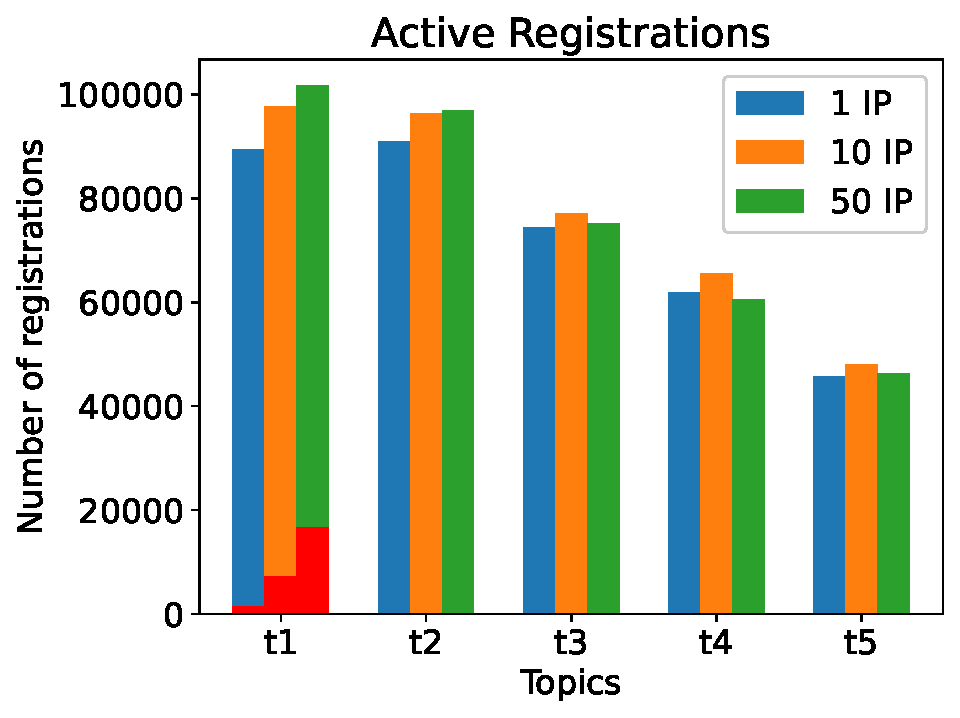
\includegraphics[width=0.22\textwidth]{img/eval/attack/registration_origin_t1.eps} 
\label{fig:reg_eclipse_t1}
} 
\hspace{-0.15cm}
\subfigure[{Active registrations eclipse attack t5 attack}]{
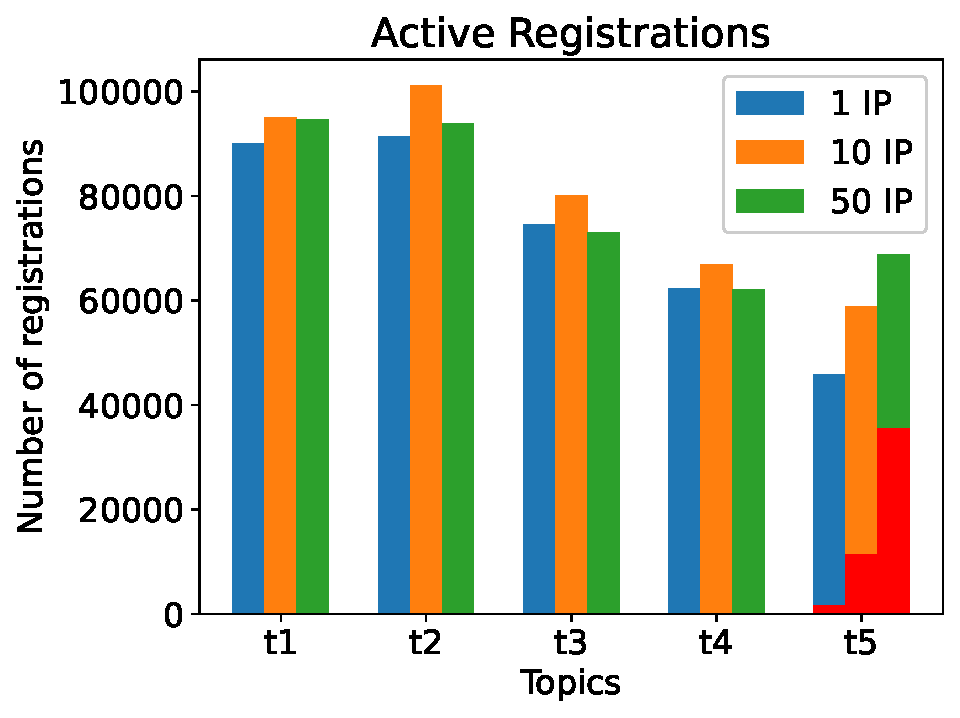
\includegraphics[width=0.22\textwidth]{img/eval/attack/registration_origin_t5.eps} %\hspace{-1.5em}%
\label{fig:reg_eclipse_t5}
}
 \caption{Active registrations under topic eclipsing attack} 
\label{fig:reg_eclipse}
\vspace{-0.15in}
\end{figure}   

In Figure~\ref{fig:reg_eclipse_t1} we observe the active registrations in the simulation per topic, for an eclipsing attack targeted to the most popular topic (t1), including active registrations of malicious nodes.
We can observe than even though the number of malicious nodes is equivalent to 20\%, the number of active registrations is lower than that. 
As expected, as the number of IP addresses used in the attack increaseas, the number of active registrations of malicious nodes also increase, since different malicious nodes with complete different IPs can not be diffierentiated from valid nodes.
For topic 5, the most vulnerable topic for being the least popular, we can observe a similar pattern of active registrations. 
However, we observe that despite malicious nodes being more (400 nodes) than valid nodes (218 nodes), active registrations of malicious nodes is kept lower than 30\% in all cases. Similarly to t1, the active registrations increase with the higher number of IPs used in the attack, since there is no way to a totally distributed attack without reusing IP addresses.


\begin{figure}[!h]
\centering
\subfigure[{Time between registration and first discovery t1 attack}]{
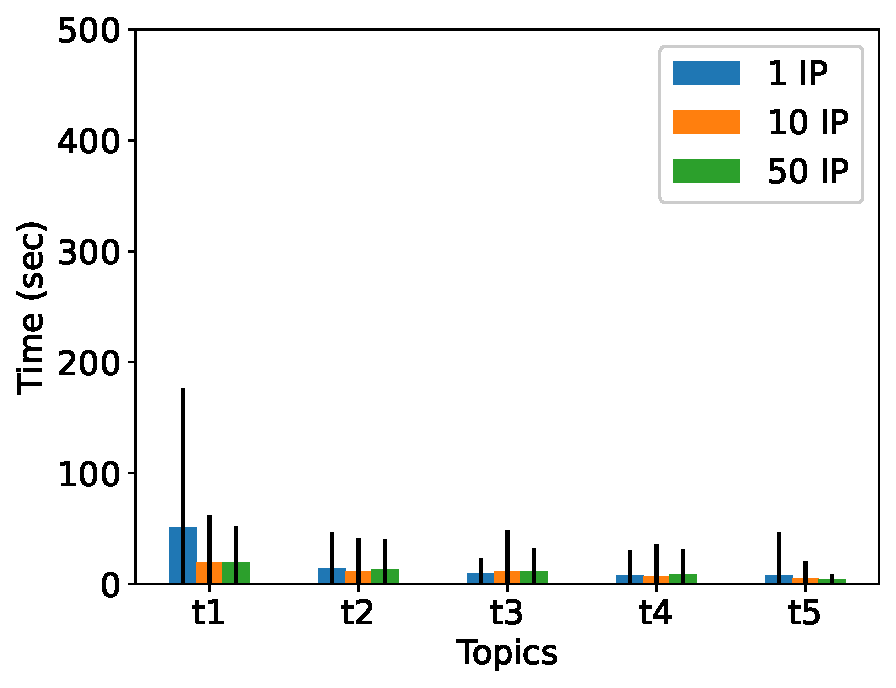
\includegraphics[width=0.225\textwidth]{img/eval/attack/min_time_discovery_t1.eps} 
\label{fig:discoverytime_eclipse_t1}
} 
\hspace{-0.16cm}
\subfigure[{Time between registration and first discovery t5 attack}]{
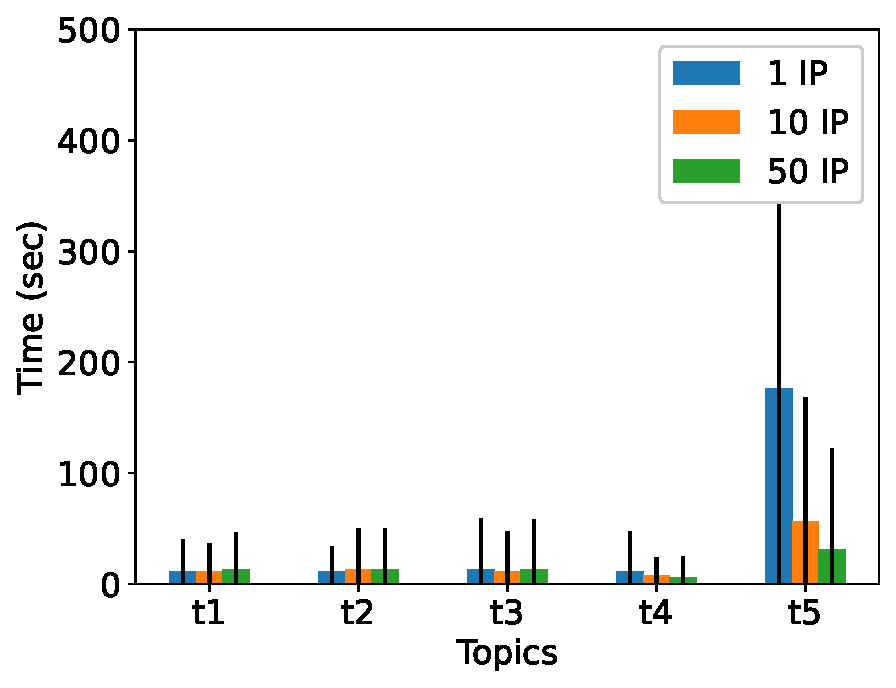
\includegraphics[width=0.225\textwidth]{img/eval/attack/min_time_discovery_t5.eps} %\hspace{-1.5em}%
\label{fig:discoverytime_eclipse_t5}
}
 \caption{Time between registration and first discovery under topic eclipsing attack} 
\label{fig:discoverytime_eclipse}
\vspace{-0.15in}
\end{figure}   

In Figure~\ref{fig:discoverytime_eclipse} we observe the average time between a node registers for a topic successfully and the node is discovered for the first time from the placed registration.
We can observe that when a topic is under attack the time required for first time discovery increases. 
This is caused by the fact that there are much more registrations in the topic caused by the attack and also that malicious nodes discovery time is higher due to the difficulty to place registrations in nodes close to the topic hash.  
We can observe that when using more IP addresses in the attack the time required to discover a node is reduced because malicious nodes are more discovered.

\begin{figure}[!h]
\centering
\subfigure[{Lookup hopcount eclipse attack t1}]{
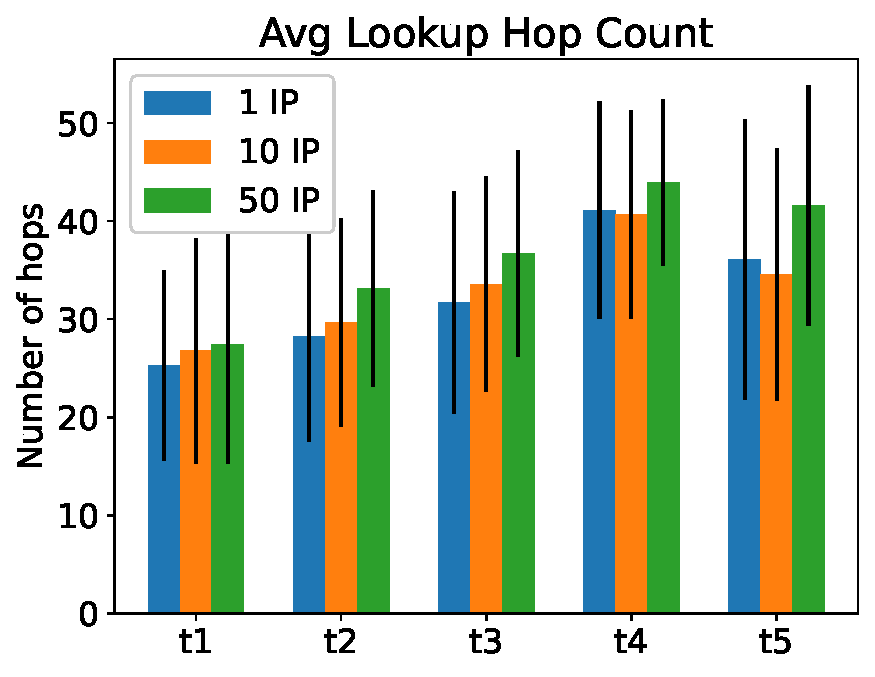
\includegraphics[width=0.225\textwidth]{img/eval/attack/lookup_hopcount_t1.eps} 
\label{fig:lookup_eclipse_t1}
} 
\hspace{-0.16cm}
\subfigure[{Lookup hopcount eclipse attack t5}]{
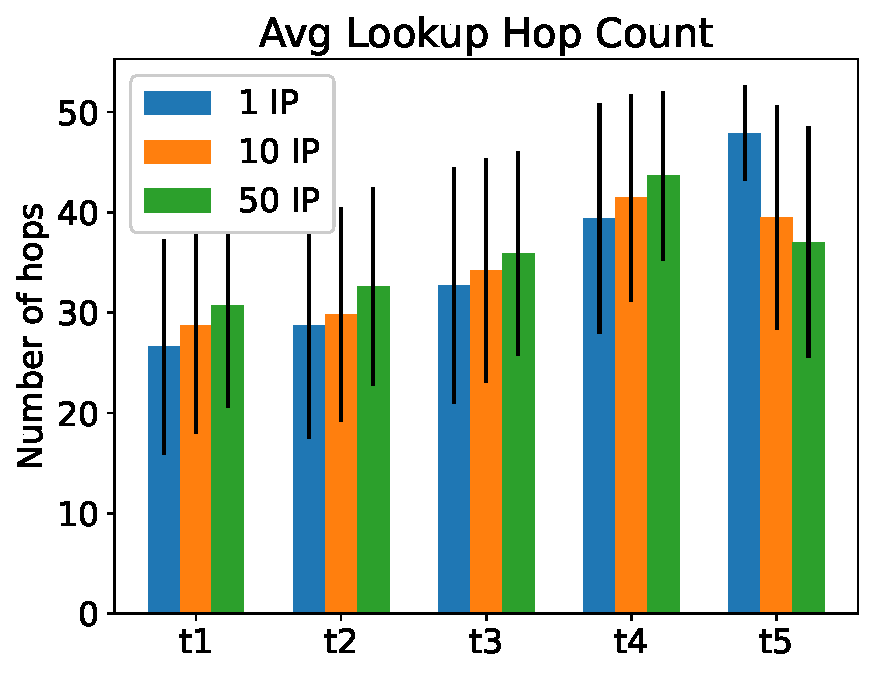
\includegraphics[width=0.225\textwidth]{img/eval/attack/lookup_hopcount_t5.eps} %\hspace{-1.5em}%
\label{fig:lookup_eclipse_t5}
}
 \caption{Lookup hopcount under topic eclipsing attack} 
\label{fig:lookup_eclipse}
\vspace{-0.15in}
\end{figure}   

\sergi{redo fig14 and fig15 figures increasing font and using eps}

In Figure~\ref{fig:lookup_eclipse} we observe the lookup hopcount in the simulation per topic,  for an eclipsing attack targeted to the most popular topic (t1) and the least popular topic (t5).
We observe that despite receiving an attack targeted at a specific topic,  the lookup performance in the network is not substantially affected by the attack.

In Figure~\ref{fig:perf_spam} we observe the performance of the topic discovery system under  the topic spam attack.
\sergi{TODO: add no sybil in the graph}
In Figure~\ref{fig:active_regs_spam} we observe the average active registrations per topic increasing the number of IP addresses used by sybil identities performing the attack.  
We observe that the number of active registrations per topic are decreased under the topic spam attack being topic 1 the most affected.
However, by observing Figure~\ref{fig:hopcount_spam} we see he lookup performance is not affected and therefore there is no substantial impact of the attack in the discovery performance of the network, concluding the system is resistant to topic spam attacks.
In Figure~\ref{fig:time_register_spam} we observe the average time required for registering for a topic,  increasing the number of Ip addresses used by sybil identities performing the attack.  
We observe again it seems there is no substantial impact of the attack to the time required to register for each topic

\sergi{add spam storage used?}

\begin{figure*}[!h]
\centering
\subfigure[{Active registrations under topic spam attack}]{
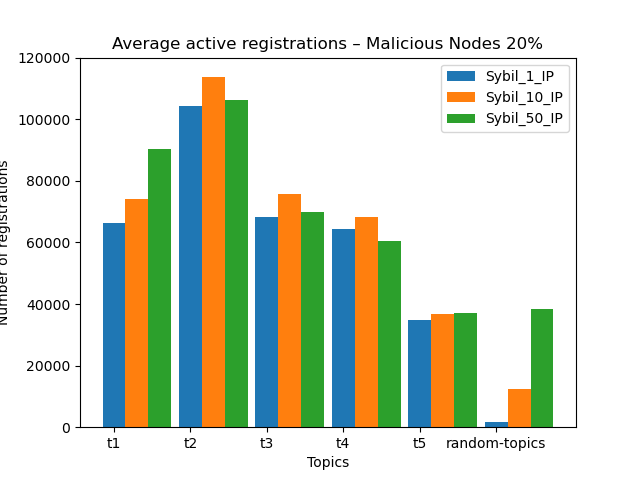
\includegraphics[width=0.275\textwidth]{img/eval/attack/registration_origin_spam.png} 
\label{fig:active_regs_spam}
} 
\hspace{-0.16cm}
\subfigure[{Time to register under topic spam attack}]{
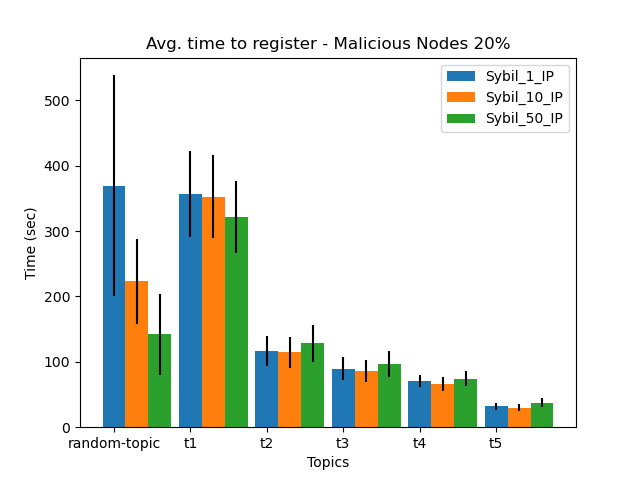
\includegraphics[width=0.275\textwidth]{img/eval/attack/avg_time_register_spam.png} %\hspace{-1.5em}%
\label{fig:time_register_spam}
}
\hspace{-0.15in}
\subfigure[{Lookup hop count topic spam attack}]{
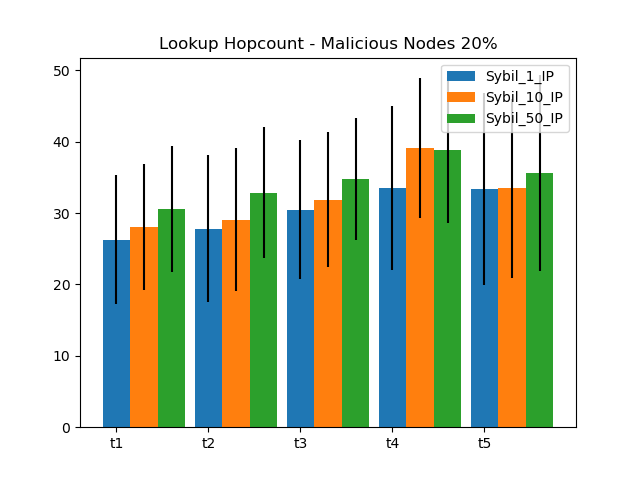
\includegraphics[width=0.275\textwidth]{img/eval/attack/lookup_hopcount_spam.png} %\hspace{-1.5em}%
\label{fig:hopcount_spam}
}
\caption{Performance evaluation topic spam attack} 
\label{fig:perf_spam}
\vspace{-0.15in}
\end{figure*}   

In Figure~\ref{fig:perf_dos} we observe the performance of the topic discovery system under the dos attack where registrars do not respond to advertisers trying to block active registrations.
In Figure~\ref{fig:active_regs_dos} we observe the average active registrations per topic increasing the number of sybil identites from 5\% to 20\% of the nodes in the network.
We observe that the number of registrations are affected by attackers,  being more affected for very popular topics,  but less affected low popularity topics.  However in none of the cases malicious nodes are able to block the active registrations and the reduction of the performance is lower than the number of sybils used.
In Figure~\ref{fig:time_register_dos} we observe the average time required for registering for a topic,  increasing the number of sybil identites from 5\% to 20\% of the nodes in the network.
We observe in this case it seems there is no substantial impact of the attack to the time required to register for each topic
In Figure~\ref{fig:time_discovery_dos} we observe the average time between an advertiser place a registration in a registrar and another node discovers it through the registrar,  increases the number sybils again.
We also observe there is no substantial impact of the attack, concluding the system is resistant to DoS attacks.

\begin{figure*}[!h]
\centering
\subfigure[{Active registrations under DoS attack}]{
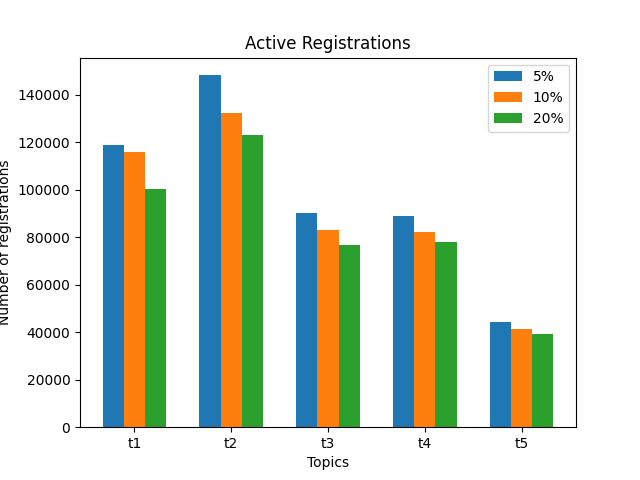
\includegraphics[width=0.275\textwidth]{img/eval/attack/registration_origin_dos.png} 
\label{fig:active_regs_dos}
} 
\hspace{-0.16cm}
\subfigure[{Time to register under DoS attack}]{
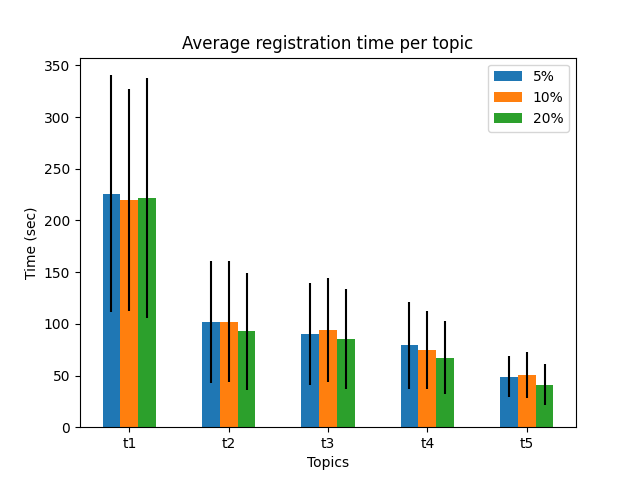
\includegraphics[width=0.275\textwidth]{img/eval/attack/avg_time_register_dos.png} %\hspace{-1.5em}%
\label{fig:time_register_dos}
}
\label{fig:discovery_dos}
\hspace{-0.15in}
\subfigure[{Time to first discovery under DoS attack}]{
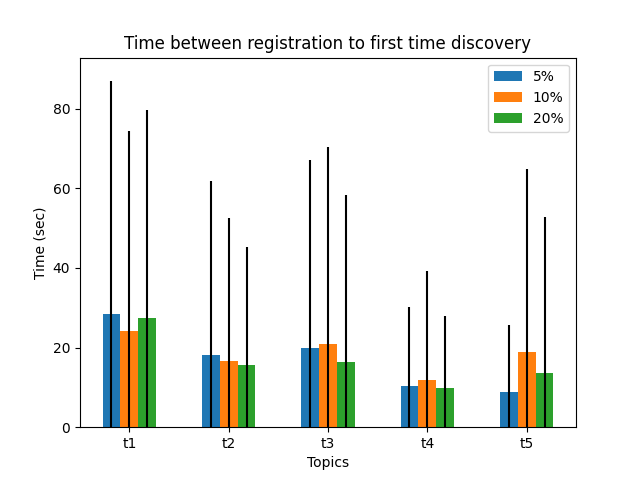
\includegraphics[width=0.275\textwidth]{img/eval/attack/min_time_discovery_dos.png} %\hspace{-1.5em}%
\label{fig:time_discovery_dos}
}
\label{fig:perf_dos}
\caption{Performance evaluation no-response DoS attack} 
\vspace{-0.15in}
\end{figure*}   


%\subsection{Testbed evaluation}
%
%"Geth"~\cite{go-ethereum} performance evaluation: \hl{TBC}.


%!TEX root = ../main.tex
%=========================================================

\section{Related Work}
\label{sec:related}

\er{Maybe discuss the byzantine-resilient peer sampling system Brahms, that also uses a blocking mechanism when more than a threshold number of view updates (pushes) are received in a certain amount of time (not sure if this is overall or for a specific node though)~\cite{}}

There exists several protocols aimed at discovery devices providing network services for local area networks.
For instance, the Simple Service Discovery Protocol (SSDP)~\hl{missing ref},  basis of the discovery protocol of Universal Plug and Play (UPnP)~\hl{missing ref},  or the DNS-based service discovery,  are used to advertise services that other devices provide,  such as printers,  webcams,  HTTPS servers, and other mobile devices,  usually using multicasting or broadcasting techniques.
However for service discovery in Internet-wide environments, since it is not possible to broadcast,
centralized setups are commonly used to provide service discovery with good performance.
UDDI~\hl{missing ref} has been recognized as the most popular discovery mechanism for
Web services.

But when focusing on decentralized architectures,  service discovery has been addressed from different perspectives. 
Most of the solutions use Distributed Hash Table (DHT) based protocols using key-based routing to discover other peers. 
CAN, Chord,  Pastry or Kademlia,  are examples of DHT protocols where all the nodes self-organize themselves into overlay networks. 
DHT-based solutions offer fault-tolerant,  scalable and efficient ways of finding nodes in large-scale networks.
However,  directly applying DHT for service discovery  present some drawbacks.
The main one is the difficulty in guaranteeing the availability of published service descriptions.
Usually,  DHT-based systems often distribute descriptions of functionally equivalent services to the same successor node,  as they have the same or similar hashing values. 
If such a node fails, a service consumer will not be able to discover any of these services. 
There are existing approaches that solve the issue. 
For instance,  Chord4S~\cite{chord4s} enhances Chord protocol by distributing service descriptions to different successor nodes. 
In case one node fails, a service consumer is still able to find functionally equivalent services that are stored at other successor nodes.

Another solution for service discovery on peer-to-peer overlay networks could be the use of topic-based pub/sub systems. 
These exists some solutions,  such as~\cite{scribe,poldercast,banno2015},  that uses DHT-based systems to multicast data to subscribers.
Similarly,  TERA~\cite{baldoni2007tera} uses topic-based pub/sub system
but using gossip protocols and self organization.  
%TERA provides a good balance between bandwidth consumption and performance guarantees. 
Similar solutions could be use to announce nodes that offer a certain service.
However,  those solutions rely on the use of rendezvous points for publishing the data,  which adds a single point of failure to the network.
Moreover,  continuous multicast of data to nodes subscribed for a service adds overhead to the network.
However,  all these solutions have not been designed with Sybil-resistance in mind and it requires that all nodes be trusted.

%"Centralized and distributed protocols for tracker-based dynamic swarm management"~\cite{dan2012centralized}


Another possible solution for service discovery in blockchain platforms is to incorporate a service discovery component to the blockchain. 
In~\cite{manevich2019endorsement}, a new service discovery component is presented for  Hyperledger Fabric (HLF),  a permissioned blockchain platform.
The service discovery component provides APIs that allow the client application to dynamically discover the configuration details of the endorsement policies and chaincode it needs to use.
However, since HLF is a smaller scale private blockchain it does not require large-scale service discovery as ours and it does not need to prevent this service discovery feature from attackers.

%"Endorsement in Hyperledger Fabric via service discovery"~\cite{manevich2019endorsement}: allows Hyperledger Fabric client to locate available services (chaincodes) using an API since HLF version 1.2. Before the set of services (chaincodes) was hardcoded at the client and server side. 
Similalry,  in~\cite{farmer2021decentralized} the authors propose decentralized identifiers for peer-to-peer service discovery.
%"Decentralized identifiers for peer-to-peer service discovery"~\cite{farmer2021decentralized}:
Besides the service discovery feature in Ethereum itself, some applications build service discovery over Ethereum, as in this example of decentralized identifiers (there are tons of examples of web services using the blockchain to store and retrieve service representatives)~\cite{keizer2021flock}.

%"Under the Hood of the Ethereum Gossip Protocol"~\cite{kiffer2021under}: a study of Ethereum gossip protocol that I did not read yet.

%Ethna~\cite{wang2021ethna} seems also similar.




%\subsection{Eclipse attacks in Eth/p2p}

%Approaches to leverage security in DHT-based networks.

In the area of avoiding Sybil and derived eclipsing attacks in peer-to-peer networks several solutions and state-of-the-art can be found in the literature.
In~\cite{danezis2005sybil},  different strategies are devised to make DHTs resilient to malicious nodes trying to poison lookups,  by routing queries in a way that minimizes trust bottlenecks,  to minimize the amount of poisoned information that honest nodes receive from adversarial nodes.
In a similar way,  S/Kademlia~\cite{skad} propose new mechanisms to get resilience against common attacks by using parallel lookups over multiple disjoint paths,  limiting free nodeld generation with crypto puzzles and introducing a reliable sibling broadcast.

In ~\cite{cholez2010efficient},  the authors propose  a statistical approach to detect a particular type of Sybil attack in  Kademlia DHT,  where Sybil peers strategically choose IDs that are close to a target ID in the DHT ID space.
The authors found that the expected the ID distribution of the closest nodes returned in the search results for target IDs follow a geometric distribution. Therefore, the divergence from geometric distribution of the node IDs in search results indicate existence of Sybil nodes in the results.  However, computing a divergence threshold is not straightforward and requires fine tuning to avoid false positives when detecting Sybil nodes.

In~\cite{marcus2018low}~and~\cite{henningsen2019eclipsing},  the authors present low-resource eclipsing attacks for the Ethereum P2P network.  
The attack ensures that the lookup-buffer used to initiate outbound connections is filled up with adversarial nodes by placing an adversarial node to each one of the DHT buckets, requiring only  2 IPs from distinct /24 subnets to be successful.
As a result of this paper, Geth v1.8 and v1.9 implemented new countermeasures,  such as  increasing number of connections, considering all nodes of the table during lookups,  or throttling the inbound connection attempt,  to reduce the chance of selecting an attacker-node .

%"Efficient DHT attack mitigation through peers' ID distribution"~\cite{cholez2010efficient} – This paper proposes a statistical approach to detect a particular type of Sybil attack in vanilla Kademlia DHT, where Sybil peers strategically choose IDs that are close to a target ID in the DHT ID space. If sufficient number of (i.e., typically 10 or more) Sybil peers are successfully placed closest to a target ID, then the Sybils could attract all or most of the search and registration requests for that ID because of their proximity to that target and launch attacks such as returning bogus search results. On the other hand, the normal behaviour of honest peers is to generate their IDs uniformly at random. Based on measurements on a DHT with only honest peers, the authors find that the expected the ID distribution of the closest nodes returned in the search results for target IDs follow a geometric distribution. Therefore, the divergence from geometric distribution of the node IDs in search results indicate existence of Sybil nodes in the results. Once divergence is detected, the IDs that contribute the most to the divergence are considered to be Sybils and are therefore omitted from the search results. However, computing a divergence threshold is not straightforward and requires fine tuning to avoid false positives when detecting Sybil nodes.


%S/Kademlia~\cite{skad}.
%"S-Kademlia"~\cite{pecori2016s}


Security lessons learned from literature:
\begin{itemize}
\item Assume that the underlying network layer does not provide any security properties to the overlay layer.
\item Importance of difficulty on generating random ids.
\item Nodes should not be capable of generating any id and duplicate ids should not be possible.  Ids should be linked to ip,  port or public key.
\item  Use of  parallel lookups over multiple disjoint paths to avoid querying only  adversarial nodes paths.
\item Importance of limiting IPs per bucket to require more resources to launch a sybil attack.
\item Avoid querying only nodes close to topic id / node id because adversarial nodes can strategically place nodes close to those ids.
\end{itemize}

%In "Eclipsing Ethereum Peers with False Friends"~\cite{henningsen2019eclipsing} - ,  the authors present  a false friends attack,  an eclipse attack applicable to Geth version v1.8.20.  The attack ensures that the lookup-buffer used to initiate outbound connections is filled up with adversarial nodes by placing an adversarial node to each one of the DHT buckets. 
%Since there is a limit that at most 2 nodes from the same /24 subnet can be included in the same bucket and at most 10 nodes from the same /24 can be in the whole table,  it requires  2 IPs from distinct /24 subnets to be successful,  and in contrast
%with previous attacks, it can be successfully mounted without
%assuming that the victim node reboots at some point, and can be completed in a matter of days.
%In response to the attack presented in the paper,  Geth version v1.9.0 implemented new countermeasures,  such as i) increasing number of connections from 25 to 50 ii) considering all nodes of the table during lookups, instead of only the bucket heads,  to reduce the chance
%of selection an attacker-node and iii) throttle the inbound connection attempts to limit the consecutive inbound connection attempts from the same IP to 30 seconds.

%"Low-Resource Eclipse Attacks on Ethereum's Peer-to-Peer Network."~\cite{marcus2018low} - 

"Sybil-resistant DHT routing"~\cite{danezis2005sybil} - they enhance standard DHT routing with information about the social network (by whom the nodes where introduced into the DHT). Based on that, they try to detect and avoid Sybils. Again, we don't have an introduction social network. 

\sergi{I haven't read these papers yet. To be included}
"A Sybil-proof one-hop DHT"~\cite{lesniewski2008sybil}

"Sybilinfer: Detecting sybil nodes using social networks."~\cite{danezis2009sybilinfer}
SybilInfer is an algorithm aimed at detecting Sybil attacks in social networks using e Bayesian inference approach.  It  labels which nodes are honest and which are dishonest with a degree of certainty. The decision is based on an analysis of social connections. However, it requires a social network that we do not have in our setup. 

"Whanau: A sybil-proof distributed hash table"~\cite{lesniewski2010whanau} - 


"Persea: a sybil-resistant social dht"~\cite{al2013persea} - 


"Design and evaluation of Persea, a Sybil-resistant DHT"~\cite{al2014design} - 

"Defending the sybil attack in p2p networks: Taxonomy, challenges, and a proposal for self-registration"~\cite{dinger2006defending}


"Quantitative analysis of the sybil attack and effective sybil resistance in peer-to-peer systems"~\cite{jetter2010quantitative}


GossipSub: Attack-Resilient Message Propagation in
the Filecoin and ETH2.0 Networks~\cite{gossipsub}


%!TEX root = ../main.tex
%=========================================================

\section{Notes}
Increase the blacklisting time to sth higher than ad\_lifetime

Introd why


Discovery - state that we do a fix betad non-



\subsection{Tasks}
Paper: 

\begin{itemize}
	\item Write abstract
    \item Complete intro
    \item Complete background
    \item Describe all the attacks we already considered (where?)
    \item complete related work
    \item complete missing references
    \item add python simulation results and scenario description in performance evaluation
    \item add security results  in performance evaluation
\end{itemize}

Other tasks:

\begin{itemize}
	\item Get past attack traces from Felix
    \item IP -> new system (done?)
\end{itemize}

\clearpage
% ========= references =========
\bibliographystyle{plain}
\bibliography{references}

\end{document}